\newpage
\vskip 6mm
\pagestyle{myheadings}
\markboth{{\underline{\centerline{东南大学博士学位论文} }}}
{{\underline{\centerline{第三章 \ \ \  基于自适应小波分解和多元核密度估计的多尺度因果推断} }}}

\chapter{基于自适应小波分解和多元核密度估计的多尺度因果推断}\label{ch3}
\setcounter{equation}{0}
 
\section{引言}
因果检测是时间序列分析的一项基本任务,旨在识别变量之间的顺序关系,强调变量之间的方向性影响\cite{3_1}。与时间序列相关分析中的对称关系不同,因果关系被定义为不对称关系\cite{3_2}。传递熵(Transfer entropy, TE)是一种显著的基于信息熵的时间序列因果检测方法,用于度量两个时间序列之间的因果关系\cite{3_3}。一般来说,从序列$X$到序列$Y$的TE表示在掌握了$X$和$Y$\cite{3_35}的历史信息后,下一个时间步预测未来值$Y$的不确定性降低。R\'{e}nyi传递熵 (R\'{e}nyi RTE) \cite{3_4}作为TE的扩展,通过参数$\alpha$既能考虑罕见事件和频繁事件,又能考虑序列中的特殊分布部分。近年来,基于RTE的多种因果检测方法在过去几十年中被提出,因为它具有分析具有不对称、时滞、间接相关甚至非线性系统的机制分析的时间序列的优势\cite{3_34}。例如,Mi等人结合振动模态分解和RTE,基于脑电图(EEG)信号探索脑电极间多层次连接状态\cite{3_5}。基于RTE和有效传递熵,He等。提出了一种有效的r\'{e}nyi传递熵来分析股票时间序列之间的信息流,可以减弱噪声对股票时间序列的影响\cite{3_6}。Armah等人提出了一种基于rte的方法来衡量发达国家房地产与政策不确定性之间的因果关系\cite{3_7}。

尽管有这些成功的先例,但在将RTE引入特定领域时仍存在一些挑战。首先,作为一种基于信息熵的模型,在计算RTE时不可避免地要计算概率密度分布,在实际中需要对其进行估计。概率密度分布估计的准确性将直接决定TE在因果检测中的有效性。一类方法是直接利用现有的观测数据,基于不同类型的估计器估计联合概率密度分布和边际概率密度分布\cite{3_8}。举几个例子,Kraskov等\cite{3_9}通过引入$k$ -最近邻来解决概率分布的局部近似,提出了互信息的估计。Faes等\cite{3_10}提出了一种基于修正条件熵估计序列间信息流的非线性格兰杰因果关系方法。上述方法虽然可以有效地估计概率密度函数,但往往需要预先定义一些超参数,并假设整个原始数据的概率密度分布。因此,RTE构造的另一个分支是基于内核密度估计(KDE) \cite{3_11}。例如,Giraldo等\cite{3_12}提出了一种基于无限可分核定义的算子在再现核希尔伯特空间中估计概率的非参数方法。在Giraldo等人\cite{3_12}的基础上,De La Pava等人\cite{3_13}提出了一种基于RTE估计的脑电信号因果检测的数据驱动测量方法,该方法提供了RTE的线性组合表达式。随后,Zhou等人通过显著性分析\cite{3_14}将KDE方法扩展到基于矩阵的RTE估计的多变量情况,既可以检测间接因果关系,也可以检测共同因果关系。因此,基于kde的方法可以通过估计RTE值而不是估计概率分布来获得更好的因果检测结果。然而,上述文献并未提供一维核方法与多维核方法之间的关系,这促使我们在单变量和多变量情况下寻求基于kde的RTE估计方法的测度统一准则。
此外,现实世界中的复杂系统通常是一个多层系统,传统的RTE无法捕获多尺度情况下的因果关系。为了解决这一问题,一些学者将小波变换(WT)作为分析非平稳信号的经典时间序列分解方法引入到因果检测中。Materassi等人基于TE和连续小波变换(CWT) \cite{3_15}研究了地球磁层尖端磁场动力学各变量之间不同频带的因果关系。Storhas等\cite{3_16}基于CWT和符号传递熵检测了原油和成品油返回动态的多尺度因果关系。此外,离散小波变换(DWT)也被用于多尺度因果检测。例如,提出了一种基于DWT和TE的因果检测方法来测量耦合系统\cite{3_31}中变量之间的信息传递。Guo等\cite{3_17}利用二进平稳小波变换将脑电图和肌电图信号分解为5个频段,应用TE检测不同时间尺度下的皮质-肌肉耦合。这些工作证明了将基于小波变换的时间序列分解引入因果检测的可行性和必要性。然而,对于离散小波,最优滤波器是非常理想的,这也会影响最终因果检测的性能。近年来,一些学者基于机器学习求解最优小波系数。Saadatmorad等人(\cite{3_18})引入卷积神经网络设计最优小波系数。Lu等人\cite{3_19}提出了一种基于小波神经网络和切换粒子群优化的混合方法,将小波系数作为待训练模型的参数。同样,Zhao等人提出了一种基于深度残差网络的方法来融合不同频段的多个小波系数,每个小波系数可以通过模型训练自适应调整\cite{3_20}。需要指出的是,上述基于机器学习的方法都需要预先定义一些超参数。因此,基于机器学习的方法在克服预定义超参数问题上还有一定的改进空间,这激发了我们去填补这一空白。

针对上述问题,本文提出了一种基于核密度估计的复杂系统因果检测新方法。该方法对各变量在不同频带上的RTE进行估计,分为两部分:基于自适应离散小波变换 (Adaptive Discrete Wavelet Transform, ADWT) 的时间序列分解部分和基于多元核密度估计(Multivariate Kernel Density Estimation, MKDE) 的RTE因果关系检测部分。ADWT模块是一个自编码器,其中编码器和解码器由同一对正交小波组成,分别对应于小波分解和重构过程。在基于adwt的时间序列分解中,系统的多变量时间序列在自编码器框架下,通过最小化原始时间序列与重构时间序列之间的均方误差(MSE)产生最优逼近系数和详细系数,在多层中将系统的多变量时间序列分解为高频分量和低频分量。每层的分量构成分量变量邻接矩阵,节点表示变量,边表示因果关系。这些变量邻接矩阵被输入到因果网络生成部分来计算因果关系。在基于MKDE的因果网络生成中,每个变量之间的因果关系用RTE值表示,RTE值由MKDE模块估计。KDE的度量是基于最小化KDE中每个变量的概率密度函数与核函数之间的渐近平均积分误差(AMISE)。本文给出了单变量和多变量情况下基于AMISE的KDE统一评价准则。此外,我们还选择了单变量和多变量核情况下的最优带宽。为了验证该方法的有效性,在合成数据和实际数据上进行了实验。结果表明,本文提出的方法基于ADWT模块和MKED模块,可以对不同频段的传输信息进行量化。与其他估计方法的比较结果表明,所提出的方法可以更准确、更显著地估计变量之间的因果关系。
\section{模型描述}
新型RTE的估计框架如图\ref{figure1}所示,它由两个模块组成:基于自适应离散小波变换(ADWT)的时间序列分解和基于多变量核密度估计(MKDE)的RTE因果关系网络生成。输入的$X\in \mathbb{R}^{m\times t}$是$m$组时间序列,$t$是每个时间序列的长度。$X$首先被送入ADWT模块以计算近似系数$H_{D}\in \mathbb{R}^{n\times\frac{t}{2}}$和详细系数$G_{D}$中。通过最小化输入数据$X$和重建数据$hat{X}$之间的均方误差(MSE),在$\mathbb{R}^{n\times \frac{t}{2}}$中获得$H_{D}$和$G_{D}$。在基于ADWT的时间序列分解模块中,原始时间序列在最优小波系数的作用下被分解为不同层的高频成分$X^{h}(n)$和低频成分$X^{l}(n)$。在基于MKDE的因果关系网络模块中,系统内各变量的因果关系由变量相邻矩阵表示。每个变量的分解分量依次形成邻接矩阵,其中最后一层的低频分量作为趋势项,形成低频分量变量邻接矩阵$G^{l}$,各层的高频分量作为波动项,形成高频分量变量邻接矩阵$G^{h}$。这些邻接矩阵作为输入进入基于MKDE的因果网络部分的生成部分。邻接矩阵的值表示变量之间的因果关系,初始值为0。变量之间的因果关系将由RTE值呈现,在每一层中,MKDE模块通过最小化概率分布和最优带宽的核函数之间的渐近平均积分误差(AMISE)来估计。最后,每层的变量邻接矩阵 $G_{n}=(V, E)$是整个模型的输出。在详细介绍所提出的方法中的两个模块之前,我们先对离散小波变换和RTE进行简单的初步介绍。

\subsection{预备知识}
\subsubsection{离散小波分解}

\begin{figure}[!htbp]
\centering
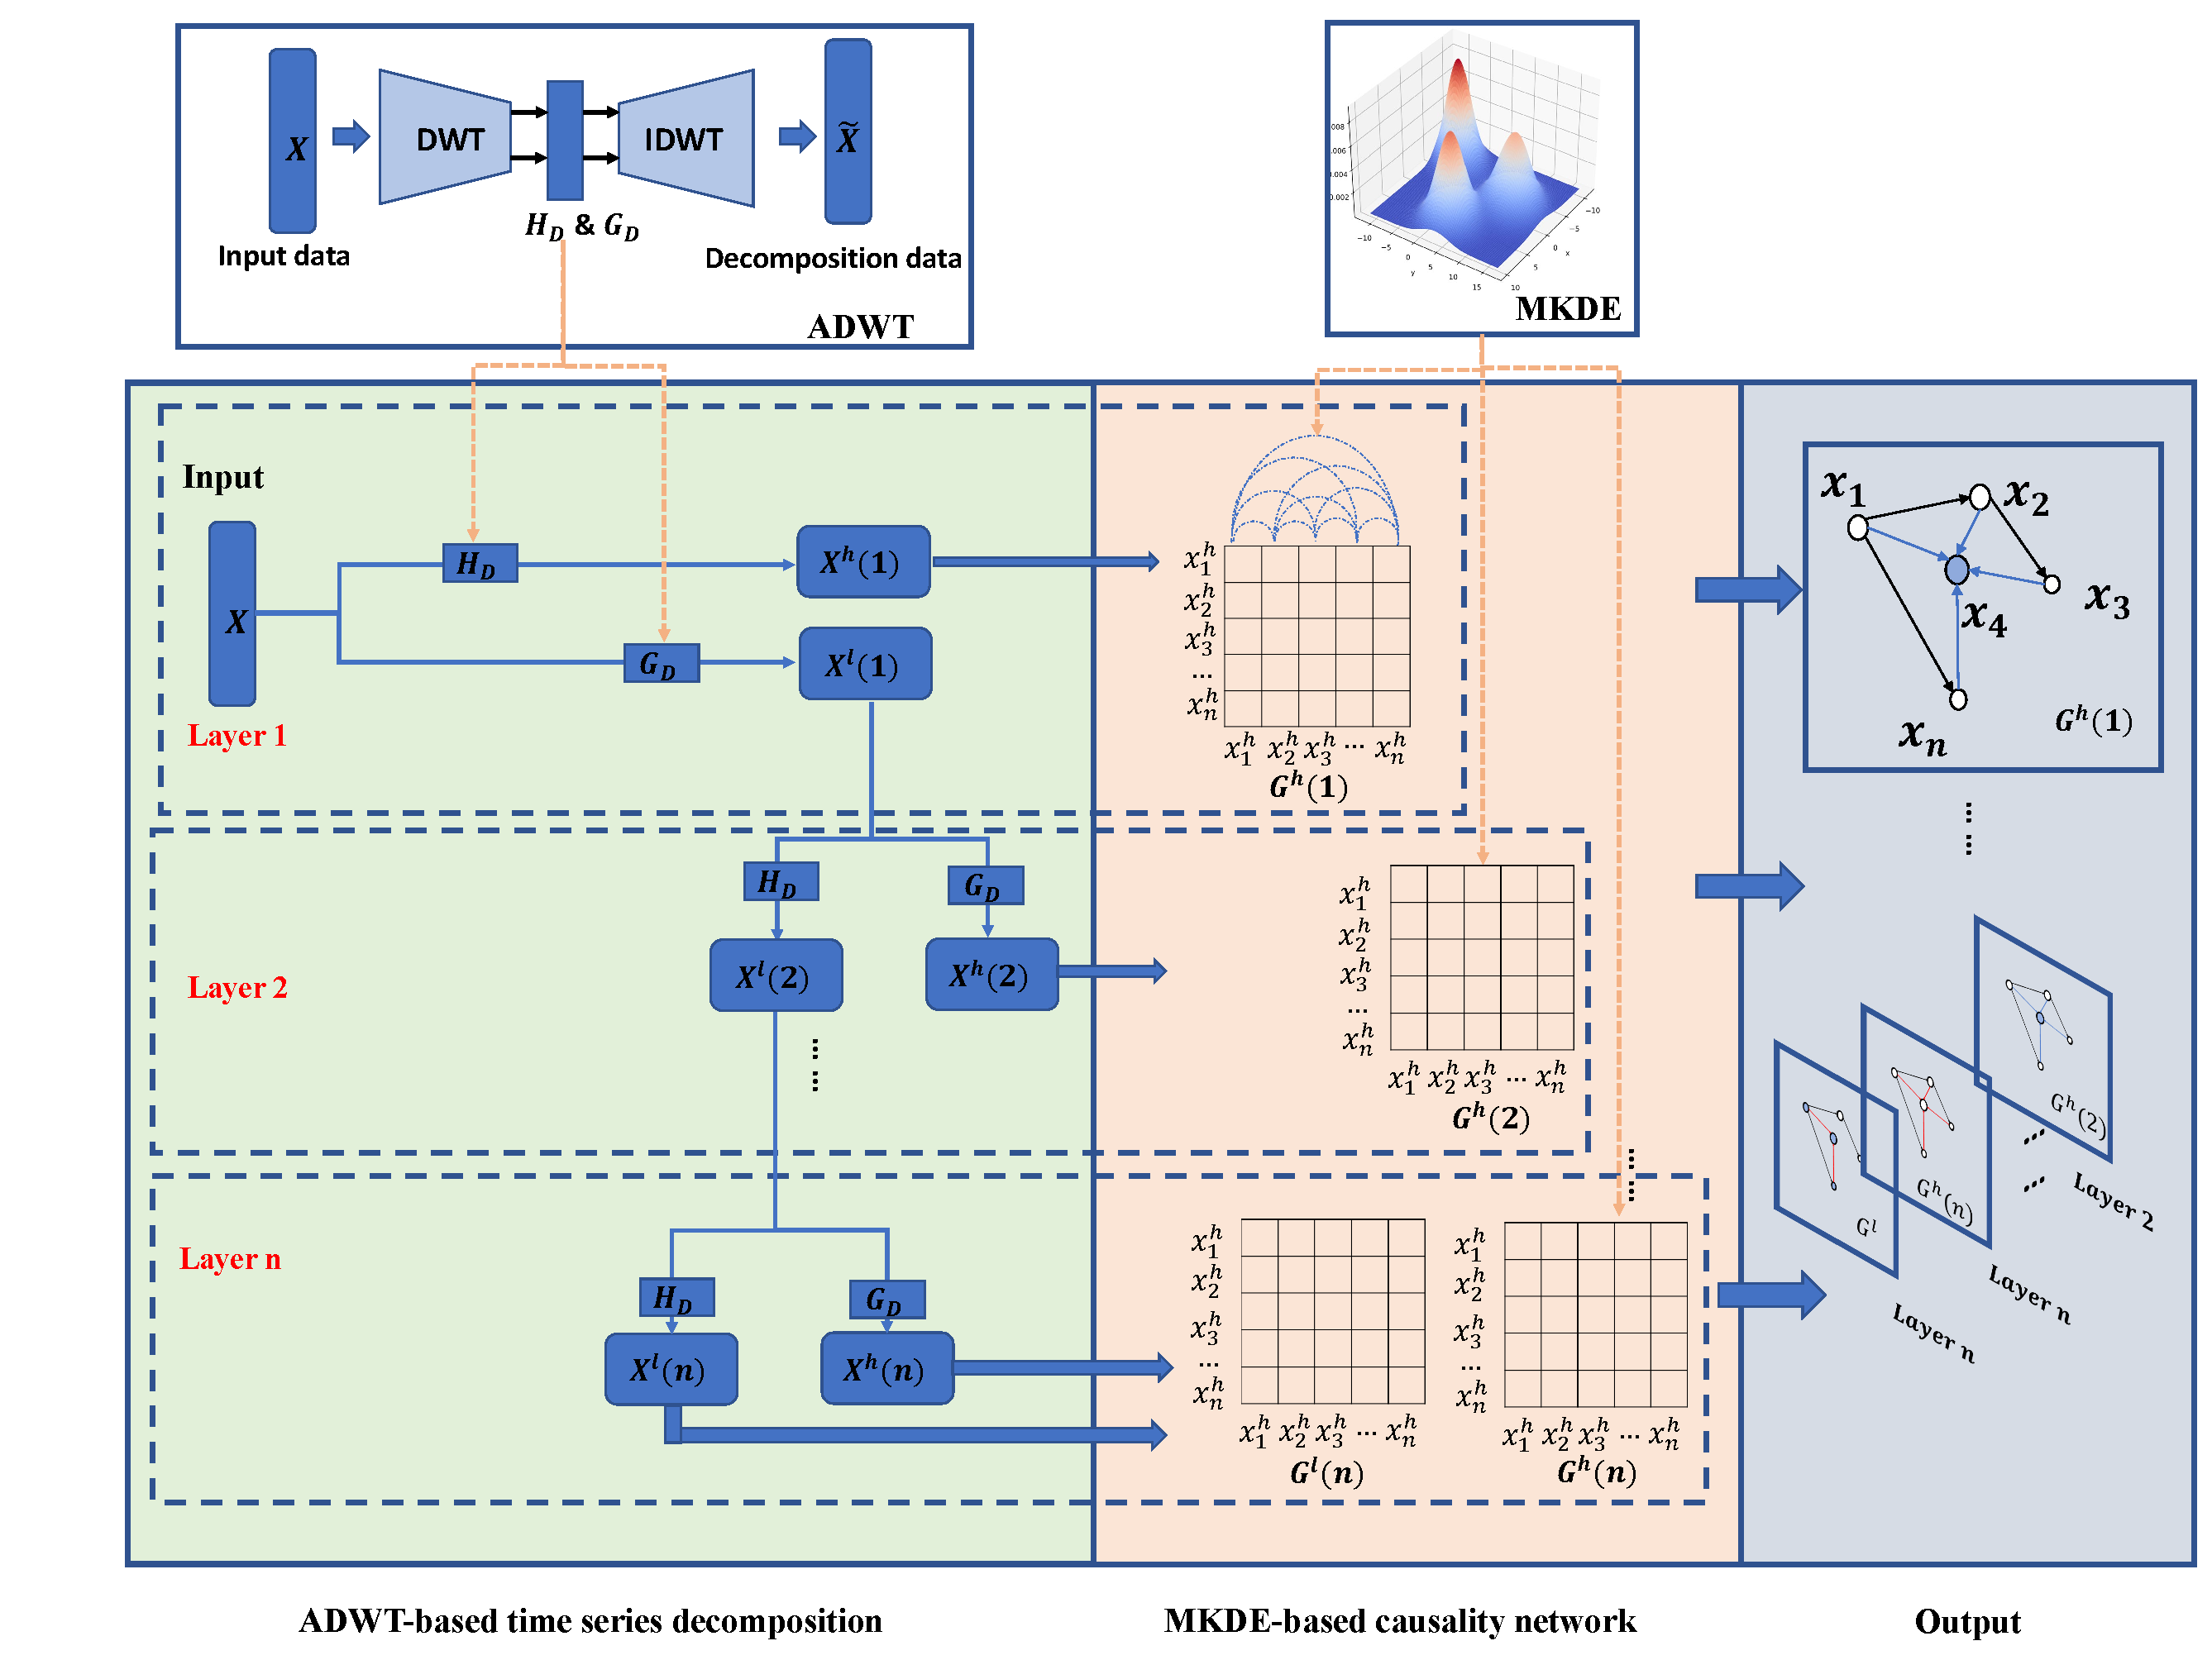
\includegraphics[scale=0.3]{./ch3/fig3_1.pdf}
\caption{新型RTE的估计框架。} \label{figure1}

\end{figure}

在现实的复杂系统中,观察结果总是以离散的形式存在,因此,通常采用DWT来捕捉时间和频率的定位。小波分解的完整框架是一个分层结构,每一层都有两个部分:时间序列分解和时间序列重构。如图中的时间序列分解部分。
图\ref{figure2},DWT通过高通滤波器$h_{i}$和低通滤波器$g_{i}$在第i层将时间序列$x^{l}_{i}$分解为高频分量和低频分量。其中,时间序列分解过程可以通过以下方式给出:
\begin{align}\label{DWT}
\begin{cases}
y^{l}_{t}(i+1)= H_{D}(M\cdot t) = \sum\limits_{t=1}^{t}x^{l}_{i}(M \cdot T -t)\cdot h_{i},\\[0.5em]
y^{h}_{t}(i+1)= G_{D}(M\cdot t) = \sum\limits_{t=1}^{t}x^{l}_{i}(M \cdot T -t)\cdot g_{i},
\end{cases}
\end{align}
其中,$y^{l}_{t}(i+1)$和$y^{h}_{t}(i+1)$是$i+1$层原始序列的$t$时间步长的低频分量和高频分量,对应于所谓的近似序列和详细序列\cite{3_21},它们代表原始序列的趋势项和波动项。此外,$x^{l}_{i}(M\cdot T -t)$是第$i$层的子序列,是对上层输出的下采样。$M$为比例因子,$T$为滤波器的分解长度。$H_{D}(t)/in h_{i}$是第$i$层的近似系数,$G_{D}(t)/in g_{i}$是第$i$层的详细系数。
在时间序列重建部分,分解后的序列可以通过反离散小波变换进行重建:
\begin{align}\label{IDWT}
y'^{l}_{i}(t) = \sum_{t=1}^{t}x^{l}_{i+1}(M \cdot T -t)\cdot h'_{i+1}+
                \sum_{t=1}^{t}x^{h}_{i+1}(M \cdot T -t)\cdot g'_{i+1},
\end{align}
其中重建滤波器$h'$和$g'$是分解滤波器的镜像函数。因此,这对重建滤波器也是正交镜像滤波器。$x(M\cdot T -t)$的作用是,在与相应的滤波器卷积之前,要重建的序列被上采样(每个元素之间插入零)。
单级DWT的图示摘要见图\ref{figure2}。该图说明了高通滤波器$h$和低通滤波器$g$对于DWT是必要的,包括过滤、下采样和上采样的因素。同时,DWT的中间结果,低频分量和高频分量可以用来表示原始序列中不同频段的特征。
\begin{figure}[!htbp]
\begin{center}
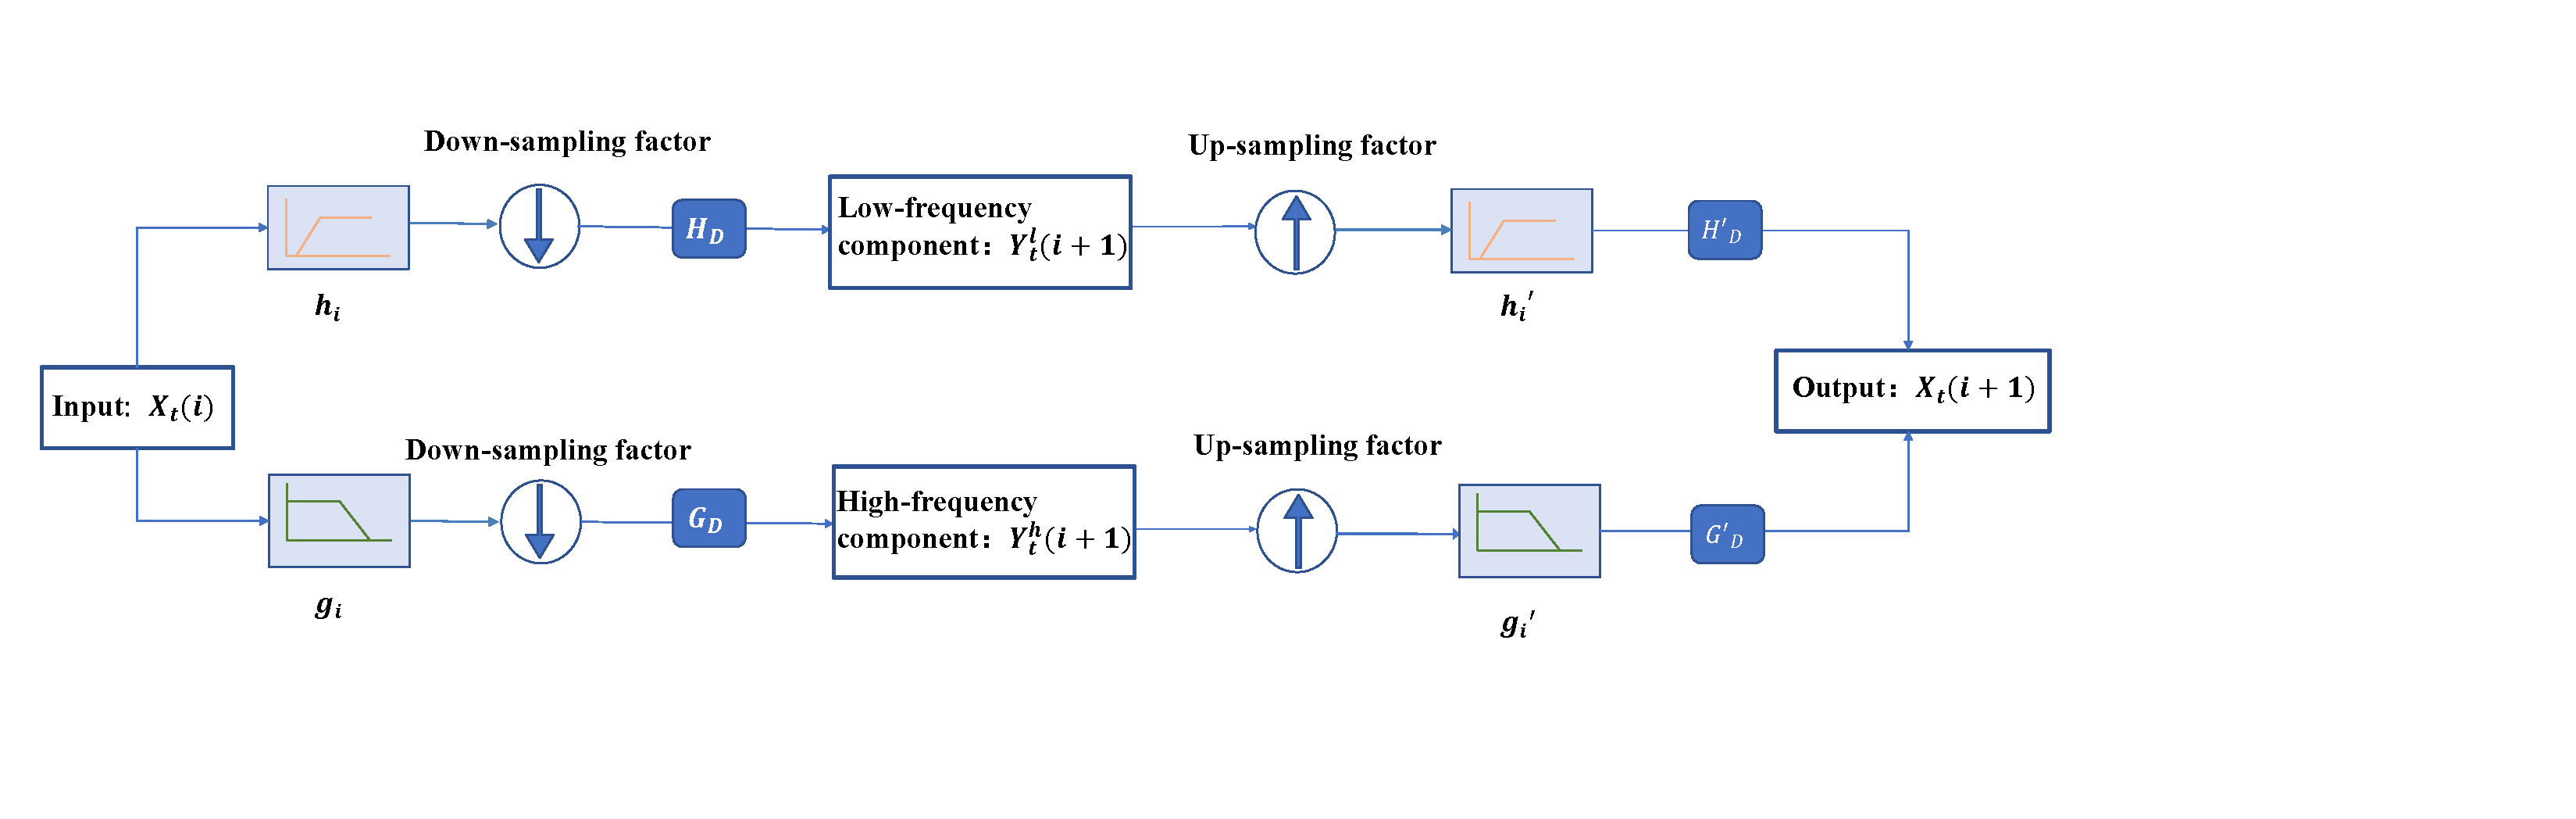
\includegraphics[width=1\textwidth]{./ch3/fig3_2.pdf}
\caption{基于单层DWT的时间序列分解和重建的图示} \label{figure2}
\end{center}
\end{figure}

\subsubsection{R\'enyi 传递熵}
R\'enyi传递熵(R\'enyi transfer entropy, RTE)是对香农传递熵(Shannon transfer entropy, STE)在复杂分布下的扩展和泛化。因此,在介绍RTE之前,先简单介绍一下STE。STE是一种基于信息论和概率论的非参数测量,用于量化系统间的传递信息和因果关系。考虑到一个复杂的系统$S$,它产生了两个离散的Markov过程$X_{t}=x_{1}, x_{2}, \ldots, x_{t}$和$Y_{t}=y_{1}, y_{2}, \ldots, y_{t}$,顺序为$k$和$l$,其中每个变量的概率分布为$p_{x_{t}}$和$p_{y_{t}}$。时间步数是离散的,单步为$tau$,$t_{n}$为未来时间步数。从$Y$到$X$的STE,即 $T_{Y\rightarrow X}(k,l)$的定义是:

\begin{align}\label{TE}
T_{Y\rightarrow X}(k,l) &\equiv I(X_{t+1}:Y_{t}^{(l)}|X_{t}^{(k)}) \notag\\
&= H(X_{t+1}:X_{t}^{(k)}) - H(X_{t+1}:(Y_{t}^{(l)}, X_{t}^{(k)})) \notag\\
&=\sum\limits_{x_{t}^{(k)} \in X_{t}^{(k)}, y_{t}^{(l)} \in Y_{t}^{(l)}} p(x_{t+1}, x_{t}^{k}, y_{t}^{l}) \log_{2}(\frac{p(x_{n+1}|x_{t}^{(k)},y_{t}^{l})}{p(x_{t+1}|x_{t}^{k})}),
\end{align}

TE在理论上等同于从$Y_{t}^{l}$到$X_{t+1}$的条件互信息,以历史序列$X_{t}^{k}$为条件, 其中$X_{t}^{k}={X_{t}, X_{t-1}, \ldots, X_{t-k+1}}$和$Y_{t}^{l}={Y_{t}, Y_{t-1}, \ldots, X_{t-l+1}}$为联合过程集合。香农传递熵(STE) (\ref{TE}) 是定量测量 $X_{n_{t+1}}$通过观察$Y_{t}$到时间$t_{n}$会减少多少不确定性的基本方法。考虑到香农熵形式$H_{s}=-\sum p(x)\rm{log}$$(p(x))$,方程(\ref{TE})也可以表示为熵形式:

\begin{align}\label{STE}
T_{Y\rightarrow X}(k,l) = H_{s}(X_{t}^{k},Y_{t}^{l})-H_{s}(x_{t},Y_{t}^{l},X_{t}^{k})+H_{s}(x_{t},X_{t}^{l})-H_{s}(x_{t}^{l}),
\end{align}
其中$H_{s}(\cdot)$和$H_{s}(\cdot, \cdot)$分别为边际熵和联合熵。
不同于SE,R\'enyi熵(RE)是一个指数加权的不确定性度量的平均值,在形式上为SE的单参数泛化。假设$\alpha>0$,具有概率分布$\mathcal{P}$的变量$X$的RE被定义为:
\begin{align}\label{RE}
H_{\alpha}[\mathcal{P}] =\frac{1}{1- \alpha}\log_{2}\sum\limits_{x\in X}p^{\alpha}(x),
\end{align}
特别是,当$\alpha=1$时,RE指的是SE。有关RE及其参数$\alpha$的性质在上一章中有过介绍,在本章中不再赘述。基于RE的引入,以及上述STE的定义(\ref{TE}),RTE可以被表达为:
\begin{align}\label{RTE}
T^{R}_{\alpha, Y\rightarrow X}(k,l) =\frac{1}{1- \alpha}\log_{2}\frac{\sum \rho_{\alpha}(x^{(k)}_{n}) p^{\alpha}(x_{n+1}|x_{n}^{(k)})}{\sum \rho_{\alpha}(x^{(k)}_{n}, y_{n}^{(l)}) p^{\alpha}(x_{n+1}|x_{n}^{(k)},y_{n}^{(l)})},
\end{align}
其中$\rho_{\alpha}(x^{k}_{n}) \equiv \frac{p^{\alpha}(x^{k}_{n})}{\sum p^{\alpha}(x^{k}_{n})}$是$x^{k}_{n}$的护送分布$(\rm{escort\ distribution})$,$\rho_{\alpha}(x^{k}_{n}, y_{n}^{l})$是$x^{k}_{n}, y_{n}^{l}$的联合护送分布$(\rm{joint\ escort\ distribution})$。RTE可以通过调整$\alpha$的值来关注概率密度函数的不同部分。特别是,对于$\alpha=1$,可以证明RE指的是SE。对于$0< \alpha<1$,像长尾事件这样的边际事件会被强调出来。对于$\alpha>1$,普遍事件将被强调。类似地,将方程(\ref{RE})代入方程(\ref{RTE}),RTE也可以被改写为熵的形式:
\begin{align}\label{RTEs}
T^{R}_{\alpha, Y\rightarrow X}(k,l) = H_{\alpha}(X_{t}^{k},Y_{t}^{l})-H_{\alpha}(x_{t},Y_{t}^{l},X_{t}^{k})
+H_{\alpha}(x_{t},X_{t}^{l})-H_{\alpha}(x_{t}^{l}).
\end{align}

\subsection{基于自编码器的自适应离散小波分解}
在预备知识中我们介绍到,DWT中的高频和低频成分是原始序列与小波系数的乘积。因此,基于DWT的时间序列分解的一个关键步骤是找到合适的高通滤波系数$H_{D}$和低通滤波系数$G_{D}$来生成子序列。本章提出了一种基于编码器-解码器的自适应离散小波变换(ADWT)来求解最优系数,它可以在没有任何超参数的情况下求解最优小波系数。本章所提出的自适应离散小波分解(Adaptive discrete wavelet decomposition,ADWT)本质上是一个自编码器,其中的编码器和解码器,分别相当于离散小波分解(\ref{DWT})和重构过程(\ref{IDWT}),分别由高通滤波器$h(t)$和低通滤波器$g(t)$组成,编码-解码器的最佳高通滤波器系数$H_{D}$和低通滤波器系数$G_{D}$被用于基于ADWT的时间序列分解中。采样系数$M=2$,在这种情况下,$h(t)$和$g(t)$都是半带滤波器,这意味着分解后的序列长度是原始序列的一半。编码器-解码器模型致力于寻找最优正交的小波滤波器$h(t)$和$g(t)$,这里,最优是指在对序列进行小波变换时,这些滤波器应该足够好,能够保留与原始序列尽可能多相同的信息。

同时,根据小波分解理论,待优化的高通滤波器和低通滤波器也必须满足以下条件:
\begin{align*}
\sum_{t}h[t]^{2} = 1,\quad
\sum_{t}h[t] = \sqrt{2},\quad
\sum_{t}g[t]^{2} = 1,\quad
\sum_{t}g[t] = \sqrt{2},\quad
g(t) = (-1)^{t}h(1-t).
\end{align*}

因此,求解高通滤波器和低通滤波器的损失函数,即最优滤波器$L_{w}(h,g)$被设计为:

\begin{align}\label{loss}
{\rm L}_{w}(h,g) = (\sum_{t}h[t]^{2} - 1)^2 + (\sum_{t}h[t] - \sqrt{2})^2
           + (\sum_{t}g[t]^{2} - 1)^2 + (\sum_{t}g[t] - \sqrt{2})^2.
\end{align}

每个项都被设定为平方项,因此损失函数是可微的,以便通过梯度下降学习参数。最终,结合重构序列与原序列之间的均方根误差,本章所提出的自适应离散小波分解模块的损失函数被设计为:
\begin{equation}\label{loss2}
\min\limits_{(h,g)} {\rm L}_{loss} = W_{1} {\rm MSE}(X,X')+W_{2} {\rm L}_{w}(h,g)+W_{3} ||H_{D}||_{1}+W_{4} ||G_{D}||_{1}.
\end{equation}
损失函数是三个部分的加权和:基于均方根误差(MSE)的重建序列和原始序列之间的估计,基于高通和损失通滤波器系数的惩罚项目,以及基于滤波器的损失函数$L_{w}(h,g)$ 的约束。其中,MSE是对原始序列$X$和通过ADWT重建的序列$X'$之间差异的一种度量:
 \begin{equation}\label{mse}
{\rm MSE}(X, X') = {\frac{1}{t}\sum\limits_{i=1}\limits^{t}(\hat{x}_{i}-x_{i})^2}.
\end{equation}
在上述工作的基础上,用于求解最优滤波器的自动编码器的步骤已经完成。然后,得到的最优滤波器系数被用来生成不同层次的系统变量的高频和低频部分,后续章节所讨论的因果关系,都是在这些层次中独立存在的。
\subsection{基于核密度估计的r\'enyi 传递熵}
在预备知识中,我们提到对于公式(\ref{RTEs}),边际熵和联合熵的估计是RTE计算的关键步骤。在本章中,我们通过核密度估计(kernel density estimation,KDE),研究多变量系统中的RTE的计算。首先,我们先研究较为简单的单变量核密度估计(Univariate kernel density estimation,UKDE)。给定一个离散随机变量$X_{t}=x_{1}, x_{2}, \ldots, x_{t}$,对$X$进行KDE的标准过程可以被定义为$\tilde{f}(x)$:
\begin{align}\label{Kernelformula}
\tilde{f}(x) =\frac{1}{t}\sum\limits^{t}_{i=1}K_{h}(x-x_{i})
            =\frac{1}{th}K\left(\frac{x-x_{i}}{h}\right),
\end{align}
其中$t$是变量的长度,$K(\cdot)$是核函数,$h>0$,作为公式的平滑参数,是带宽。$K_{h}(\cdot)$是以$h$为比例因子的比例核函数。一般来说,核函数决定了概率密度函数的形状,它应该满足以下特性。
\begin{description}
  \item[1. 非负性:] $K(x)>0, \forall x \in D_{K}$;
  \item[2. 对称性:] $K(x) = K(-x), \forall x \in D_{K}$;
  \item[3. 实值性:] $K(x) \in \mathbb R, \forall x \in D_{K}$;
  \item[4. 归一性:] $ \int K(x) dx = 1, \forall x \in D_{K}$;
  \item[5. 有界性:] $\int x^{p}K(x)dx = 0, \int x^{p+1}K(x)dx = k < \infty$.
\end{description}

KDE的本质是将输入的数据和带宽作为核函数的参数,从而得到几个核函数,例如、 高斯核函数: $k(x,x')=e^{-\frac{||x-x'||^{2}}{2\sigma^{2}}}$,其中$x'$是核函数的中心,$||x-x'||^{2}$是向量$x$和$x'$之间的欧氏距离(L2 范数),而 $\sigma$控制高斯核函数的范围,$\sigma$值越大,高斯函数的局部范围越大。高斯核函数值随着两个向量之间的距离增加而单调地减少。此外,内核密度估计函数是基于内核函数的线性求和和归一化得到的。理论上,所有满足函数在定义域上的积分为1的平滑函数都可以作为KDE的核函数。由于高斯核较为典型的数学特性,因此在过往的研究中都使用高斯核对KDE的数学性质进行讨论。因此在本章中,我们选择高斯核进行后续讨论。

带宽$h$是KDE性能的另一个重要因素。带宽反映了整个KDE曲线的平坦程度,也量化了观察到的数据点在KDE曲线形成过程中的比例。带宽越大,观察到的数据点在最终曲线形状中的比例越小,整体KDE曲线越平坦;带宽越小,观察到的数据点在最终曲线形状中的比例越大,KDE曲线越陡峭。在公式(\ref{Kernelformula})中,对于输入数据$x_{i}$,给定带宽$h$,KDE函数在$x_{i}$处形成的曲线函数为 $\frac{1}{th}K(\frac{x-x_{i}}{h})$, 其中内核函数的内部$h$用于调整KDE曲线的宽度,而内核函数的外部$h$则用于确保KDE函数积分为1。容易看出,对于$n\rightarrow \infty$,带宽$h\rightarrow 0$。

接下来是关于为给定的系列样本量选择最佳带宽的讨论。我们首先关注MSE,以衡量概率密度函数$f(x)$和其估计值$hat{f}(x)$之间的均方根误差${\rm MSE}(\hat{f}(x), f(x))$:
\begin{align}\label{MSEforrmula}
{\rm MSE}(\hat{f}(x), f(x)) &= E(\hat{f}(x)-f(x))^{2}\notag\\
            &=E(\hat{f}(x) - E\hat{f}(x) +E\hat{f}(x) -f(x))^{2}\notag\\
            &=E(\hat{f}(x) - E\hat{f}(x))^{2}+E(\hat{f}(x) -f(x))^{2}\notag\\
            &={\rm var} (\hat{f}(x)) + {\rm bais}^{2}(\hat{f}(x)),
\end{align}
从上式可以看出,KDE的均方根误差${\rm MSE}(\hat{f}(x), f(x))$是关于$x$的函数,它由方差项(标准误差)和偏差组成。在此基础上,我们将其扩展至对所有由$\hat{f}(x)$组成的核函数的整体准确性的测量,即平均分级平方误差(mean intergraded squared error,MISE):
\begin{align}\label{MISEforrmula}
{\rm MISE}(\hat{f}(x), f(x)) &= E\int\limits_{-\infty}^{+\infty}(\hat{f}(x)-f(x))^{2}\notag\\
            &=\int\limits_{-\infty}^{+\infty}{\rm MSE}(\hat{f}(x), f(x))\notag\\
            &=\int\limits_{-\infty}^{+\infty}{\rm var} (\hat{f}(x)) + \int\limits_{-\infty}^{+\infty}{\rm bais}^{2}(\hat{f}(x)).
\end{align}
将KDE公式(\eqref{Kernelformula})代入上述两项,并假设概率密度函数$f(x)$至少是二阶可推导的,对其进行二阶泰勒展开,就可以得到:
\begin{align*}
{\rm var} (\hat{f}(x)) &=\frac{1}{th}\int\limits_{-\infty}^{+\infty}K^2dx-\frac{1}{t}\int\limits_{-\infty}^{+\infty}f^{2}(x)dx + o(t^{-1}+h^{4}),\\[0.5em]
{\rm bais}(\hat{f}(x))  &=\frac{h^{2}}{2}(\int\limits_{-\infty}^{+\infty}x^{2}K)\int\limits_{-\infty}^{+\infty}(f(x)'')dx + o(h^{2}).
\end{align*}
因此,对于$X$整体分布进行估计所使用的$hat{f}(x)$的整体准确性度量$\rm{MISE}(\hat{f}(x),f(x))$可以表示为:
\begin{align}\label{MISEforrmula1}
{\rm MISE}(\hat{f}(x), f(x)) = \frac{1}{th}\int\limits_{-\infty}^{+\infty}K^2dx-\frac{1}{t}\int\limits_{-\infty}^{+\infty}f^{2}(x)dx + \frac{h^{4}}{4}(\int\limits_{-\infty}^{+\infty}x^{2}K)^{2}\int\limits_{-\infty}^{+\infty}(f(x)'')^{2}dx +o(t^{-1}+h^{4}),
\end{align}
并且从上式显然得,当$t\rightarrow \infty$时,且$h\rightarrow 0$时,$\rm{MISE}(\hat{f}(x),f(x))$=0,并且$th\rightarrow \infty$。

由此,我们可以求解最佳带宽(optimal bandwidth)。进一步,我们定义渐进平均综合平方误差(asymptotic mean integrated squared error,AMISE)为:
\begin{align}\label{AMISEforrmula}
{\rm AMISE}(\hat{f}(x), f(x)) = \frac{1}{th}\int\limits_{-\infty}^{+\infty}K^2dx-\frac{1}{t}\int\limits_{-\infty}^{+\infty}f^{2}(x)dx + \frac{h^{4}}{4}(\int\limits_{-\infty}^{+\infty}x^{2}K)^{2}\int\limits_{-\infty}^{+\infty}(f(x)'')^{2}dx.
\end{align}
假设核函数$K$的属性1-5成立,它表明$ {\rm MISE}(\hat{f}(x), f(x)) = {\rm AMISE}(\hat{f}(x), f(x)) + o(t^{-1}+h^{4})$。那么,通过微分公式(\ref{AMISEforrmula}),寻找使$\rm{MISE}(hat{f}(x), f(x))$最小化的最佳带宽$h_{opti}$的问题被转化为寻找$\rm{AMISE}(\hat{f}(x), f(x))$的极值点:
\begin{align}\label{AMISEforrmula1}
 \frac{\partial {\rm AMISE}}{\partial h}= -\frac{1}{(th)^{2}}\int\limits_{-\infty}^{+\infty}K^2dx+ h^{3}(\int\limits_{-\infty}^{+\infty}x^{2}K)^{2}\int\limits_{-\infty}^{+\infty}(f(x)'')^{2}dx,
\end{align}
使上面的方程等于0,然后求解,可得:
\begin{align}\label{unvariate_case}
h_{opti} = \left(\frac{1}{t}\frac{\int\limits_{-\infty}^{+\infty}K^2dx}{\int\limits_{-\infty}^{+\infty}x^2Kdx \int\limits_{-\infty}^{+\infty}(f(x)'')^{2}dx}\right)^{\frac{1}{5}},
\end{align}
将高斯核$K$代入方程\ref{unvariate_case}中,最优带宽为
\begin{align}\label{bandwithopti1}
h_{opti} = \left(\frac{4}{3t}\right)^{\frac{1}{5}}\sigma \approx\frac{1.06\sigma}{t^{5}},
\end{align}
其中$\sigma$是样本的方差,在方程(\ref{bandwithopti1})提供的最佳带宽选择下,我们容易得到,当$t\rightarrow\infty$时,则$h\rightarrow 0$,且当$AMISE \rightarrow$ 0,$th\rightarrow \infty$。

值得注意的是,在上述讨论中,只有带宽$h$被认为是衡量估计结果的一个指标。然而,核函数的选择对估计结果也有影响,但一般认为,带宽对估计效果的影响更大,而核函数的选择一般不影响估计结果的误差范围。因此,在AMISE的讨论中我们只给出了关于带宽参数的讨论。

\subsubsection{多变量核密度估计}
在上一节中,对于具有一维核函数的单变量KDE,我们得到了最佳带宽$h$。然而,有一些多变量的联合概率项,例如: $p(x_{t+1}| x_{t}^{(k)},y_{t}^{l}) = \frac{p(x_{t+1}, x_{t}^{(k)},y_{t}^{l})}{p(x_{t}^{(k)},y_{t}^{l})}$。在RTE中,其边际概率与核估计器一致:
\begin{align}\label{marginal}
\begin{cases}
\tilde{f}(x_{t+1},x_{t},y_{t}) =\frac{1}{th_{u}}\sum\limits^{t}_{i=1}\mathcal{K}(\frac{u-u_{i}}{h_{u}})=\frac{1}{th_{x}^{2}h_{y}}\sum\limits^{t}_{i=1}K_{x}^{2}(\frac{x-x_{i}}{h_{x}})^{2}K_{y}(\frac{y-y_{i}}{h_{y}}),\\[0.5em]
\tilde{f}(x_{t},y_{t}) =\frac{1}{th_{u}}\sum\limits^{t}_{i=1}\mathcal{K}(\frac{u-u_{i}}{h_{u}})=\frac{1}{th_{x}h_{y}}\sum\limits^{t}_{i=1}K_{x}(\frac{x-x_{i}}{h_{x}})K_{y}(\frac{y-y_{i}}{h_{y}}),
\end{cases}
\end{align}
其中核函数$\mathcal{K}(u)$是乘法核:$\mathcal{K}(u)=K(u_{1})\times\ K(u_{2})\times\cdots \times\ K(u_{d})$。在将核函数从单变量扩展到多变量的情况下,会出现一些重要的差异,因此,在这里我们选择使用乘法核。在等式左边的部分,我们主要关注MKDE的公式和最佳带宽选择。
首先,类似于一维空间中的核估计器,我们定义高维空间中概率密度函数$f_{H}(x)$的一般核估计器为:
\begin{align}\label{MKernelformula}
\tilde{f}_{H}(x) =\frac{1}{t}\sum\limits^{t}_{i=1}K_{H}(x-X_{i})
            =\frac{1}{tH}K\left(\frac{x-X_{i}}{H}\right),
\end{align}
其中带宽矩阵$H \in \mathbb{H}^{d\times d}$,是一个$d$阶对称正定矩阵,$K$是一个$d$变量球形对称密度函数,$K_{H}(x) = |H|^{-\frac{1}{2}}K(|H|^{-\frac{1}{2}}x)$是带宽比例核函数。可以注意到,带宽矩阵控制了多变量KDE中核函数的带宽和方向,这与单变量情况下的一维核不同。在本文中,RTE的估计只与两个变量$X$和$Y$有关,因此我们将注意力转向双变量的情况$(d=2)$。综上,多变量核函数估计的MISE可以写成:
\begin{align}\label{MMISEformula}
{\rm MISE}(\hat{f}_{H}(x), f_{H}(x)) = E\int\limits_{-\infty}^{+\infty}(\hat{f}_{H}(x)-f_{H}(x))^{2}
=\int\limits_{-\infty}^{+\infty}{\rm var} (\hat{f}_{H}(x)) + \int\limits_{-\infty}^{+\infty}{\rm bais}^{2}(\hat{f}_{H}(x)).
\end{align}
与单变量的情况一样,多变量核函数估计的MISE也可以分解为变化项和偏置项:${\rm var}\ (\hat{f}_{H}(x))$ 和 ${\rm bais}\ (\hat{f}_{H}(x))$。对这两项进行二阶泰勒展开,我们得到:
\begin{align}\label{Mvar_baisforrmula}
\begin{cases}
{\rm var} (\hat{f}_{H}(x)) =\frac{1}{t\mathop{\rm{det}}({\mathbf{H}})}\Vert{\mathcal{K}\Vert^{2}_{2}}f_{H}(x) + o(t^{-1}H^{-\frac{1}{2}}),\\[0.5em]
{\rm bais}(\hat{f}_{H}(x))=\frac{1}{2}\mu_{2}(\mathcal{K})
\int\limits_{-\infty}^{+\infty}[\hbox{tr}\{\mathbf{H}^{\top}\mathcal{H}_{f}(x)\mathbf{H}\}]dx
+ o(\Vert H\Vert ^{2}),
\end{cases}
\end{align}
其中$\Vert{\mathcal{K}\Vert^{2}_{2}}$是$\mathcal{K}$的$d-$维的$L_{2}$范数, $\mu_{2}(\mathcal{K}) I_{d}=\int\limits_{-\infty}^{+\infty} x^{\top}x\mathcal{K}(x) dx $,而 $I_{d}$是$d-$维单位矩阵, $\mathcal{H}_{f}(x)$是函数${f}_{H}(x)$的Hessian矩阵。$\hbox{tr}\{\cdot\}$是该矩阵的秩。同样的,为了求解最优带宽,我们需要令多变量核函数估计的AMISE为0。在这里$\rm{AMISE}(\hat{f}_{H}(x), f_{H}(x))$被定义为:
\begin{align}\label{MAMISEforrmula}
{\rm AMISE}(\hat{f}_{H}(x), f_{H}(x)) = \frac{1}{t\mathop{\rm{det}}({\mathbf{H}})}\Vert{\mathcal{K}\Vert^{2}_{2}}f(x)
+ \frac{1}{4}\mu^{2}_{2}(\mathcal{K})\int\limits_{-\infty}^{+\infty}
[\hbox{tr}\{\mathbf{H}^{\top}\mathcal{H}_{f}(x)\mathbf{H}\}]^{2}dx.
\end{align}

多变量情况下的MISE和AMISE的关系可以写成:$${\rm MISE}(\hat{f}_{H}(x), f_{H}(x)) = {\rm {\rm AMISE}}(\hat{f}_{H}(x), f_{H}(x)) + o(t^{-1}H^{-\frac{1}{2}}+\Vert H\Vert ^{2})$$。并且从中可以得出,当$t\rightarrow \infty$时,那么$\frac{1}{t\mathop{\rm{det}}({\mathbf{H}})}\Vert{\mathcal{K}\Vert^{2}_{2}}f(x)\rightarrow 0$。至此,本文完成了基于AMISE的单变量和多变量情况下的KDE的统一度量,现在我们转向寻求MKDE的最佳带宽矩阵。

与单变量的情况不同,最佳带宽矩阵的计算与矩阵$H$的形式有关。根据矩阵的形式,带宽矩阵可以分为三类:
\begin{description}
  \item[$\mathbf{I}$. Positive scalars times the identity matrix:] $\mathbf{H} =
            \begin{bmatrix}
            h^{2} & 0\\
            0 & h^{2}
            \end{bmatrix}$

  \item[$\mathbf{D}$.  Siagonal positive definite matrix:] $\mathbf{H} =
            \begin{bmatrix}
            h_{1}^{2} & 0\\
            0 & h_{2}^{2}
            \end{bmatrix}$
  \item[$\mathbf{F}$.  Symmetric positive definite matrix:] $\mathbf{H} =
            \begin{bmatrix}
            h_{1}^{2} & h_{1}h_{2}\\
            h_{1}h_{2} & h_{2}^{2}
            \end{bmatrix}$
\end{description}
在第一类矩阵$\mathbf{I}$中,带宽矩阵是最简单的情况,即,核函数在坐标方向上的传播具有相同的平移量,但这在实际场景中是一个过于严格的条件。在第二种情况下$\mathbf{D}$,带宽矩阵是一个对角线带宽矩阵,它对应于具有坐标方向和不同平移量的核函数。在第三种情况$\mathbf{H}$中,带宽矩阵$\mathbf{F}$是最一般的情况,它允许核函数在任意方向和平移量上移动,\cite{3_22}。

对于第一类矩阵$\mathbf{I}$,其最优带宽矩阵是一个对角阵,对角线元素即为每个单元最优带宽。由于多元核密度估计的AMISE与未知的$f_{H}(x)$有关,所以$\mathbf{D}$和 $\mathbf{F}$类的最佳带宽不能直接计算。我们引入了经验法则的带宽选择方法,它首先用于$\mathbf{I}$类矩阵,计算$\mathbf{F}$类矩阵的最优带宽。在经验法则的带宽选择中,多变量高斯分布$N(\mu, \Sigma)$的概率密度函数通常被用来作为多变量情况下的参考分布候选。不失一般性,考虑将高斯分布$N(0, I)$作为多变量情况的参考分布,其概率密度函数$f_{\mathcal{K}}$,其中核函数$\mathcal{K}$是多变量高斯核:  $\mathcal{K} = K_{Gaussian}(x_{1})\times K_{Gaussian}(x_{2})\times \cdots \times K_{Gaussian}(x_{n})$。在这种情况下,我们有 $\mu_{2}(\mathcal{K}) = 1, \Vert{\mathcal{K}\Vert^{2}_{2}}=2^{-d}\pi^{\frac{-d}{2}}$。那么方程\eqref{MAMISEforrmula}中的第二个项可以写成:
\begin{align*}
\int\limits_{-\infty}^{+\infty}[\hbox{tr}\{\mathbf{H}^{\top}\mathcal{H}_{f}(x)\mathbf{H}\}]^{2}dx
=\frac{1}{2^{d}\pi^{\frac{d}{2}}\rm{det}(\Sigma)^{\frac{1}{2}}}[2\hbox{tr}(\mathbf{H}^{\top}
\mathcal{H}_{f}(x)\mathbf{H})^{2}+\{\hbox{tr}\mathbf{H}^{\top}\mathcal{H}_{f}(x)\mathbf{H}\}^{2}],
\end{align*}
其中$\Sigma$是方差矩阵。这个结果表明,AMISE的经验法则公式与 $\mathbf{H}$和$\Sigma$的估计有关。考虑到最简单的情况,即$\mathbf{I}$类矩阵,其中 $\mathbf{H}$和$\Sigma$是对角矩阵:$\mathbf{H}=\rm{diag} (h_{1},\ldots,h_{i},\ldots,h_{d})$和$\Sigma=\rm{diag}(\sigma_{1}, \ldots, \sigma_{i}, \ldots, \sigma_{d})$。与单变量情况下的结果\eqref{unvariate_case}类似,对角线矩阵的最佳带宽为$\tilde{h}_{i}=(\frac{4}{d+2}t)^{\frac{1}{d+4}}\sigma_{i}$。根据\cite{3_24}变换,第一个因子总是在0.923和1.059之间,本文将其取为1。对于$\mathbf{D}$和$\mathbf{F}$类矩阵,我们通过将$\mathbf{I}$类中的$\Sigma$替换为其估计值$\tilde{S}$,即样本方差矩阵,可以得到MKDE的最优带宽如下:

\begin{align}\label{oprimalbandmatrix11}
\tilde{\mathbf{H}}= t^{-\frac{1}{d+4}}\tilde{S}.
\end{align}

值得注意的是,方程式\eqref{oprimalbandmatrix11}相当于对数据应用了Mahalanobis转换,将估计的协方差矩阵转换为一个单位方阵。基于最佳带宽矩阵,可以计算出来自样本随机变量的概率密度分布的估计。至此,我们就可以确定核函数并对RTE进行有效估计。



\section{实验结果及讨论}\label{c}

\subsection{数据简介}
为了确定所提出的方法的有效性,我们使用合成和真实的数据集进行了全面的评估。合成数据集包括Henon映射模型和多元回归模型,而真实数据集的来源是公开可用的因果推断开放数据库,特别是混凝土抗压强度数据集和电力负荷数据集。此外,我们还采用了一个私有的领域数据集,即沥青路面结构的RIOHTrack数据集,可以通过指定网站访问: \url{https://www.roadsdata.cn/pages/zhuantifuwu/zuchihuandao_1/kexueshuju/index.html}。这些数据的细节将在本节的其余部分提供。

\subsubsection{多元H\'{e}non映射}
H\'{e}non映射是一种经典的离散时间动态系统,可以产生混沌现象。本文使用的多变量H\'{e}non映射公式如下:
\begin{align*}
\begin{cases}
x_{t+1}=1 - ax^{2}_{t} + y_{t},\\[0.5em]
y_{t+1}=bx_{t}+cy_{t},\\[0.5em]
z_{t+1}=dx_{t}+ey_{t},
\end{cases}
\end{align*}
其中$x$,$y$和$z$为状态变量,参数设置为$a=1.4$,$b=c=0.3$、$d=0.5$和$e=0.5$,初始值设置为$x_{0}=0.1$、$y_{0}=0.1$和$z_{0}=0.1$。

\subsubsection{多变量自回归交互移动平均模型}
多变量自回归交互移动平均(Multivariate Autoregressive Interacted Moving Average,ARIMA)模型常用于非平稳时间序列数据建模。本文使用的多变量ARIMA模型有以下三个变量:
\begin{align*}
\begin{cases}
X_{t}= [Wx_{t}+(1-W)y_{t}]+\varepsilon_{X_{t}},\\[0.5em]
Y_{t}= [(1-W)x_{t}+Wy_{t}]+\varepsilon_{Y_{t}},\\[0.5em]
Z_{t}= W_{x}X_{t}+W_{y}Y_{t}+\varepsilon_{Z_{t}},
\end{cases}
\end{align*}

其中, $\varepsilon\sim N(0,1)$是白噪声,$W\in [0,1]$是耦合系数,而关于$x$和$y$的自相关方程可以被写作:
\begin{align}\label{mVAR_var}
\begin{cases}
x_{t+1} =\sum\limits_{n=1}^{\infty}a_{n}(d_{x})x_{t-n},\\[0.5em]
y_{t+1} =\sum\limits_{n=1}^{\infty}a_{n}(d_{x})y_{t-n},
\end{cases}
\end{align}
其中,$n$为滑动窗口的大小,$d\in(0,0.5)$为与Hurst系数相关的记忆参数,$a_{n}(d)$为权重系数,定义为$a_{n}(d)=d\frac{\Gamma(n-d)}{\Gamma(1-d)\Gamma(n+1)}$,$\Gamma$为伽马函数。耦合系数$W$设为0.5,初始值设为$x_{0}=0.1$和$y_{0}=0.1$。

\subsection{基准数据集CauseEffectPairs}
CauseEffectPairs数据集由从不同领域(如气象学、生物学、医学、工程学、经济学等)的37个数据集中选取的100个不同因果对的数据组成,旨在为评估因果关系发现的可信度。我们选取了其中两组多元数据,分别是混凝土抗压强度(concrete compressive strength)和电力负荷(electricity load)。混凝土抗压强度数据集是CauseEffectPairs(\cite{3_25})中的一组开放数据集,可在UCI机器学习资源库中获取。该数据集来自于混凝土抗压强度及其多元影响因素建模研究(\cite{3_26})。除混凝土抗压强度外,变量还包括水泥、高炉矿渣、粉煤灰、水、超塑化剂、粗骨料、细骨料和混凝土龄期。每个变量有1030个数据点,我们选取前800个数据点进行实验,并将其分为4组。

电力负荷是另一组来自CauseEffectPairs数据集的数据,用于研究城市电力负荷变换的多元因果关系(\cite{3_25})。该数据集是基准的第94-96对,其中三个变量是小时数、摄氏度温度和每小时兆瓦的用电量。每个变量有9504个数据点。本文选取前8000个数据点,分成10组,每组800个数据点。
\subsection{RIOHTrack数据集}
有关RIOHTrack数据集的背景及具体信息在之前的章节已经介绍过,这里不再过多赘述。这里主要探究本章所提出的自适应多层次r\'{e}nyi传递熵在路面车辙及其影响因素之间的因果检测性能。车辙数据来自RIOHTrack数据集。车辙是指在温度、湿度等环境因素的影响下,沥青路面面层在车辆荷载作用下出现的路面沟槽现象。除了车辙,RIOHTrack还提供了其他影响因素的观测:环境温度、交通和中心点挠度(CPD)。车辙和三个变量定期采集,采集周期定义为荷载车辆累计行驶里程20000km。其中,环境温度是RIOHTrack气象站在一个时期内的平均温度。由于沥青材料在高温下最易发生变形,因此采用日最高温度代表日温度。在RIOHTrack上施加的交通荷载是从2016年12月开始的挂车荷载,交通荷载的观测值是一个加载周期内的累计荷载。此外,RIOHTrack还提供了路面弯沉盆的中心点挠度,即由落锤式挠度仪(FWD)产生的沥青路面整体结构的垂直位移。作为表征路面结构刚度的重要指标,中心点挠度被认为是路面车辙性能的影响因素。迄今为止,RIOHTrack已经收集了144组有效数据。为了用更精细的观测数据计算因果关系,我们对原始数据进行了上采样,通过线性插值将数据点增加到288个。插入值基于各维度邻域基本真实值的线性插值。上采样数据按年份分为两组,选取前144个数据点,即2017年至2018年的观测数据作为第一阶段的数据,选取其余数据点,即2019年至2021年的观测数据作为第二阶段的数据。在每个阶段,数据点被分为4组,每组有36个数据点。

\subsection{结果及分析}
为了验证本章所提出的方法在发现复杂系统中各变量时间序列之间因果关系方面的有效性,我们在上述合成数据和真实数据上进行了一些实验,实验结果将在本节的其余部分提供。

\subsubsection{仿真数据实验}
仿真数据实验包括两个部分:对基于AWDT的时间序列分解模块的性能验证和对基于MKDE的因果关系检测性能验证。在第一个部分中,AWDT模块的度量指标是原始序列$X$与AWDT重建序列$\tilde{X}$之间的均方误差MSE,定义为 : $MSE(X,\tilde{X}) = \frac{1}{n}\sum\limits^{n}\limits_{i=1}(X_{i}-\tilde{X}_{i})^{2}$. $70\%$的数据用于AWDT模块中自编码器的训练,其余$20\%$的数据用于模型测试。在第二个部分中,为了验证因果关系检测的有效性,从$X$到$Y$的RTE值在噪声和时延的影响下并不是唯一的。因此,需要判断RTE值在统计上是否显著大于0。根据\cite{3_29}方法的建议,本章采用马尔可夫块引导法(Markov block bootstrap)进行显著性检验,显著水平设置为$5\%$四分位数($p<0.05$),每个block大小为20。此外,根据\cite{3_30}的建议,方程\eqref{TE}中的Maekov阶数设置为$l=k=5$。

\textbf{结果 1 : 多元h\'{e}non映射}
在基于AWDT的时间序列分解模块中,一个影响因素是分解层数。为了避免过多分解造成的计算成本,实验中将分解层设置为2。本实验以不同的初始值重复多次。以$x_{0}$, $y_{0}$, $z_{0}$为例,两层分解结果如图\ref{figure3}所示。图中从上到下依次为:原始数据、第二层产生的低频分量、第一层产生的高频分量、第二层产生的高频分量。对于每个变量,最后一层产生的低频分量表示序列的趋势,高频分量表示序列波动变化的细节,第二层的高频分量保留了更多的细节信息。可以明显看出,两级 DWT 可以从 h\'{e}non 图中得到各频段的序列特征。作为对比,我们选择了另一种基于深度残差网络(DRN)的最优小波系数方法作为对比基准模型。表\ref{table1}总结了不同初始小波函数下基于不同方法重构时间序列的平均MSE。
\begin{figure}[!ht]
\begin{center}
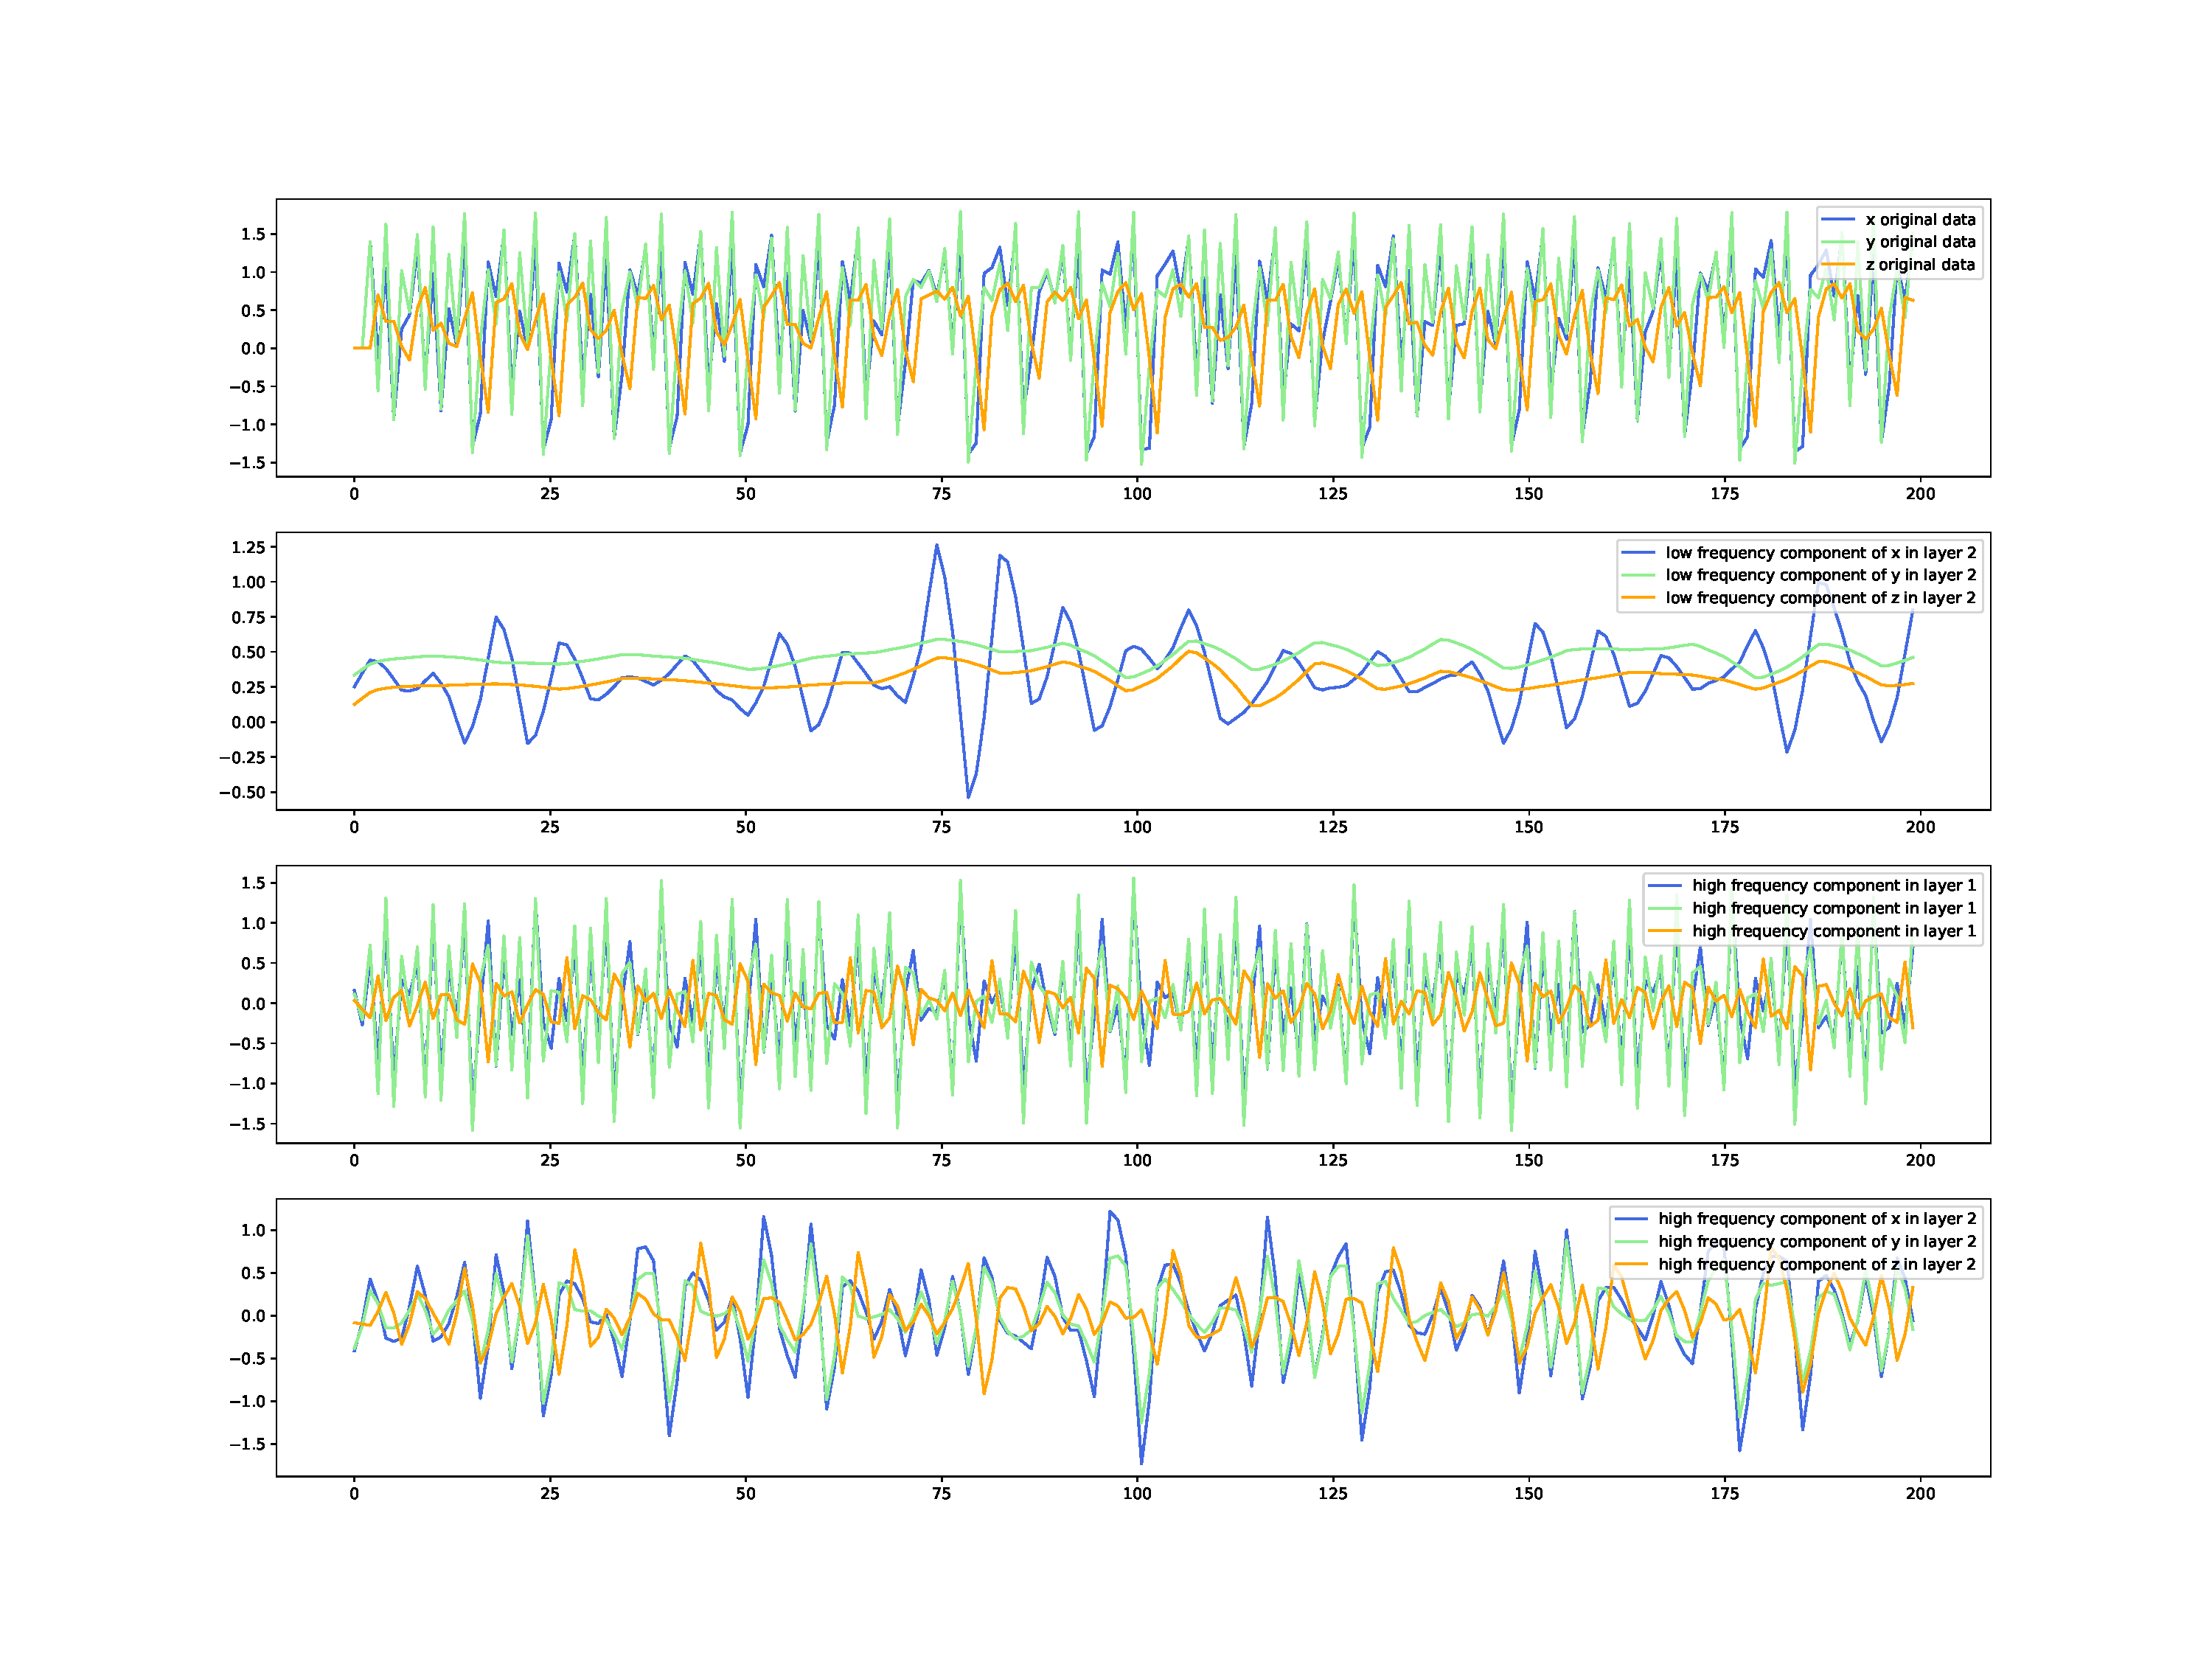
\includegraphics[width=1\textwidth]{./ch3/fig3_3.pdf}
\caption{利用ADWT模块对h\'{e}non映射中的序列进行db20小波分解。} \label{figure3}
\end{center}
\end{figure}

\begin{table}[!ht]
\fontsize{8}{12}\selectfont
\centering
\caption{Average MSE of the time series reconstruction for Henon map. The values in parentheses are the standard deviation of performance.}
\begin{tabular}{llll}
 \hline
  Wavelet function & original wavelet coefficient&  DRN based wavelet coefficient &  ADWT based wavelet coefficient \\
  \hline
  Haar & $0.4139\ (0.1164)$ & $0.3482\ (0.0446)$& $0.2731\ (0.0311)$ \\
  \hline
  db4 & $0.3579\ (0.2416)$ & $0.3095\ (0.1601)$& $0.2125\ (0.0191)$\\
  \hline
  db20 & $0.2582\ (0.0735)$ & $0.2246\ (0.0275)$& $0.1315\ (0.0305)$\\
  \hline
  Symlets4  & $0.3263\ (0.1537)$ & $0.2554\ (0.0150)$& $0.1752\ (0.0251)$\\
  \hline
  Symlets20  & $0.2471\ (0.0437)$ & $0.1722\ (0.0341)$& $0.1539\ (0.0217)$\\
  \hline
\end{tabular}
\label{table1}
\end{table}

候选小波包括Haar小波、Daubechies(dbN)小波和Coiflets小波。所有候选小波应满足正交性、规则性和长度限制。一般来说,基于ADWT模块生成的小波系数和基于DRN的小波系数在时间序列重构上的表现优于原始小波系数,基于编码器-解码器框架的ADWT模块可以在h\'{e}non映射的序列上找到离散小波分解的最优系数,并且对初始值没有约束。特别是,相较于原始小波系数基于Symlets4的ADWT模块性能提升最大;而重构后的序列在Symlets20小波上的性能最好,即重构序列于原始序列之间差异最小。同时,分解结果与消失矩和对称性(即非线性相位)有关,具体来说,db小波的特点是消失矩的阶数随阶数$N$的增大而增大,消失矩越大,平滑度越好,频域定位能力越强。Haar小波是db小波族的一个特例,小波函数在支持集上是离散的矩形波,支持集为$N=1$。symeltN是由dbN修改而来的近似对称小波。在高消失矩的小波函数的性能方面,基于ADWT的时间序列重构的性能略优于基于DRN基准方法。在消失矩较小的小波函数中,基于ADWT方法的性能提升更为明显,这说明本文方法能够以较小的计算代价获得较好的小波系数。总结来说,上述结果说明了ADWT模块在h\'{e}non映射的序列分解及重构上的有效性和鲁棒性。

基于ADWT模块的验证结果,我们继续验证基于MKDE的因果检测模块在不同频率层的有效性。从公式\ref{RTE}可知,参数$\alpha$是对RTE估计值的另一个影响因素。在这里,$\alpha$分别取$0.5$、$1$、$1.5$和$2$。基于MKDE的因果关系结果于参数$\alpha$的关系如\ref{figure4}所示。左图是在已知变量$Z$的情况下,从变量$X$到变量$Y$的RTE估计值。右图是已知变量$Z$的情况下,从变量$Y$到变量$X$的RTE估计值。x轴代表参数$\alpha$值,y轴代表分解层数,z轴代表RTE值。一般来说,$X$和$Y$之间存在双向的显著因果关系,这表明变量之间的因果关系取决于这些变量是否在一个动态系统中,而不是取决于序列之间的相似性。从参数$\alpha$的角度来看,RTE值随着$\alpha$的增大而减小,说明因果关系逐渐趋近于高概率随机事件。从分解层的角度看,信息在$X$和$Y$之间同时传递。从分解层的角度看,信息在$X$和$Y$之间同时传递,对应于低频分量的L2层的信息量从$X$传递到$Y$,再从$Y$传递到$X$是最大的,而H1层的RTE值在两个方向上都是最小的。这一结果与RTE的结论相吻合,即低频分量的因果关系受长尾事件的影响更大,而高频分量的因果关系受普遍事件的影响更大。至此,本章所提出方法的两个模块在h\'{e}non映射上的性能验证,即对基于AWDT的时间序列分解模块的性能验证和对基于MKDE的因果关系检测性能验证,已全部完成。
\begin{figure}[!ht]
\begin{center}
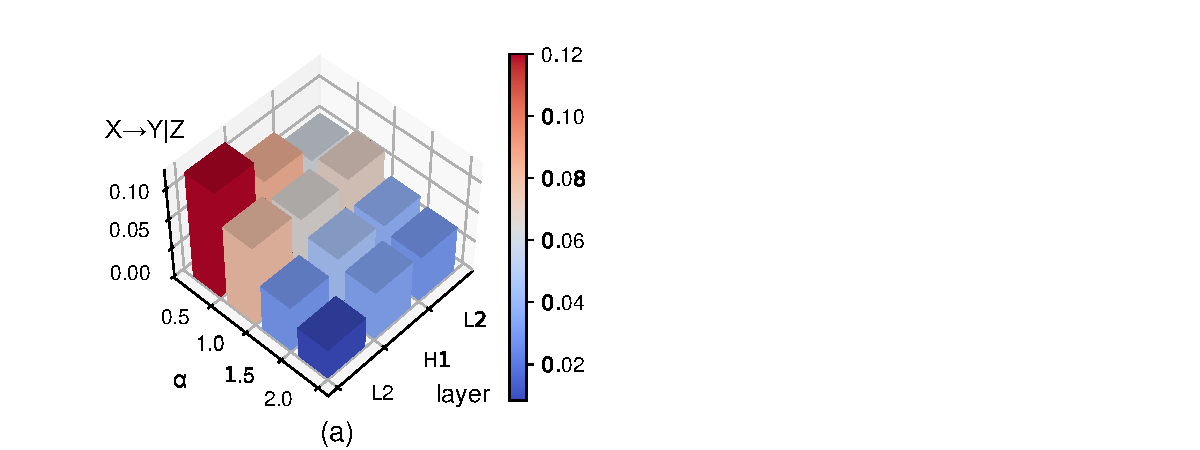
\includegraphics[scale=0.5]{./ch3/fig3_4.pdf}
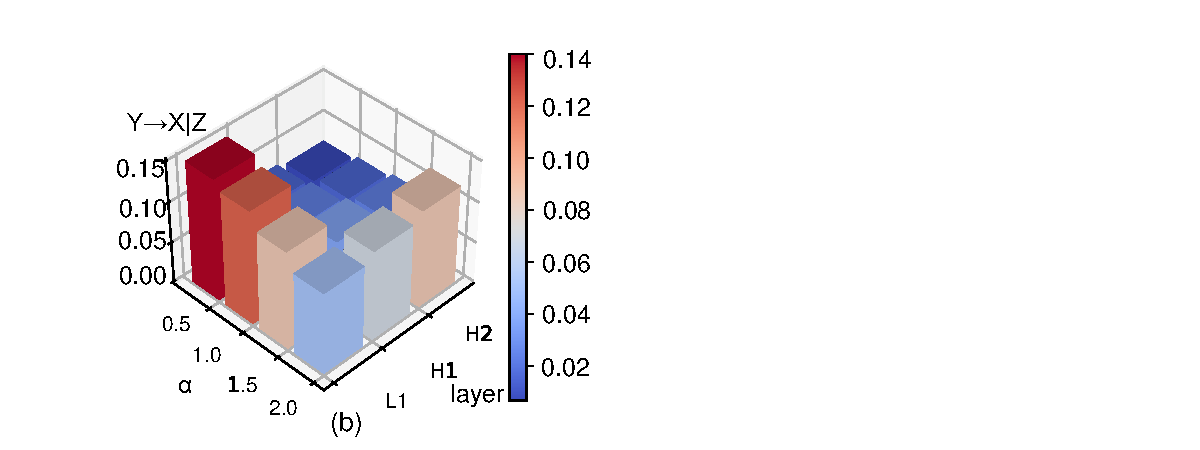
\includegraphics[scale=0.5]{./ch3/fig3_5.pdf}
\caption{基于MKDE的RTE在h\'{e}non映射上结果随参数$\alpha$的和分解层数变化的可视化。 } \label{figure4}
\end{center}
\end{figure}

\textbf{结果 2 : 多元自回归模型}
在第二个实验中,我们将使用mVAR模型生成数据继续验证所提出方法的有效性。同样,实验的目的是验证ADWT模块的性能和MKDE模块的性能。表\ref{table2}总结了基于不同小波系数生成方法的mVAR时间序列重构的性能。
\begin{table}[!ht]
\fontsize{8}{14}\selectfont
\centering
\caption{Average MSE of the ADWT module for mVAR model. The values in parentheses are the standard deviation of performance.}
\begin{tabular}{llll}
 \hline
  Wavelet function & original wavelet coefficient &  DRN based wavelet coefficient &ADWT based wavelet coefficient\\
  \hline
  Haar & $0.3751\ (0.1817)$ & $0.3370\ (0.0681)$ & $0.3091\ (0.0010)$\\
  \hline
  db4 & $0.3528\ (0.1258)$ & $0.3193\ (0.0730)$& $0.3094\ (0.0541)$\\
  \hline
  db20 & $0.2736\ (0.0288)$ & $0.2433\ (0.0052)$& $0.2018\ (0.1355)$\\
  \hline
  Symlets4  & $0.3193\ (0.1306)$& $0.2791\ (0.0680)$& $0.2373\ (0.0446)$\\
  \hline
  Symlets20  & $0.2122\ (0.0857)$ & $0.1736\ (0.0529)$& $0.1757\ (0.0836)$\\
  \hline
\end{tabular}
\label{table2}
\end{table}

从表\ref{table2}可知,与原始小波系数相比,使用ADWT模块重构的时间序列的mse在所有重构精度上都有所提高,结果更加稳健。以Symlets20与ADWT的分解结果为例,初始值为$X(0)$、$Y(0)$和$Z(0)$,如图\ref{figure6}所示。从各变量的低频成分来看,本文采用的mVAR模型中的序列呈现出明显的上升趋势。mVAR模型的性能表明ADWT模块在面对非平稳序列时具有良好的鲁棒性。特别是,由于初始小波的重构性能已经足够好,高阶消失矩小波的 ADWT 性能改善不大。因此我们可以得出结论,ADWT模块的性能提升并不适用于所有情况,有必要先使用初始小波进行对比来避免计算成本的浪费。
\begin{figure*}[!ht]
\begin{center}
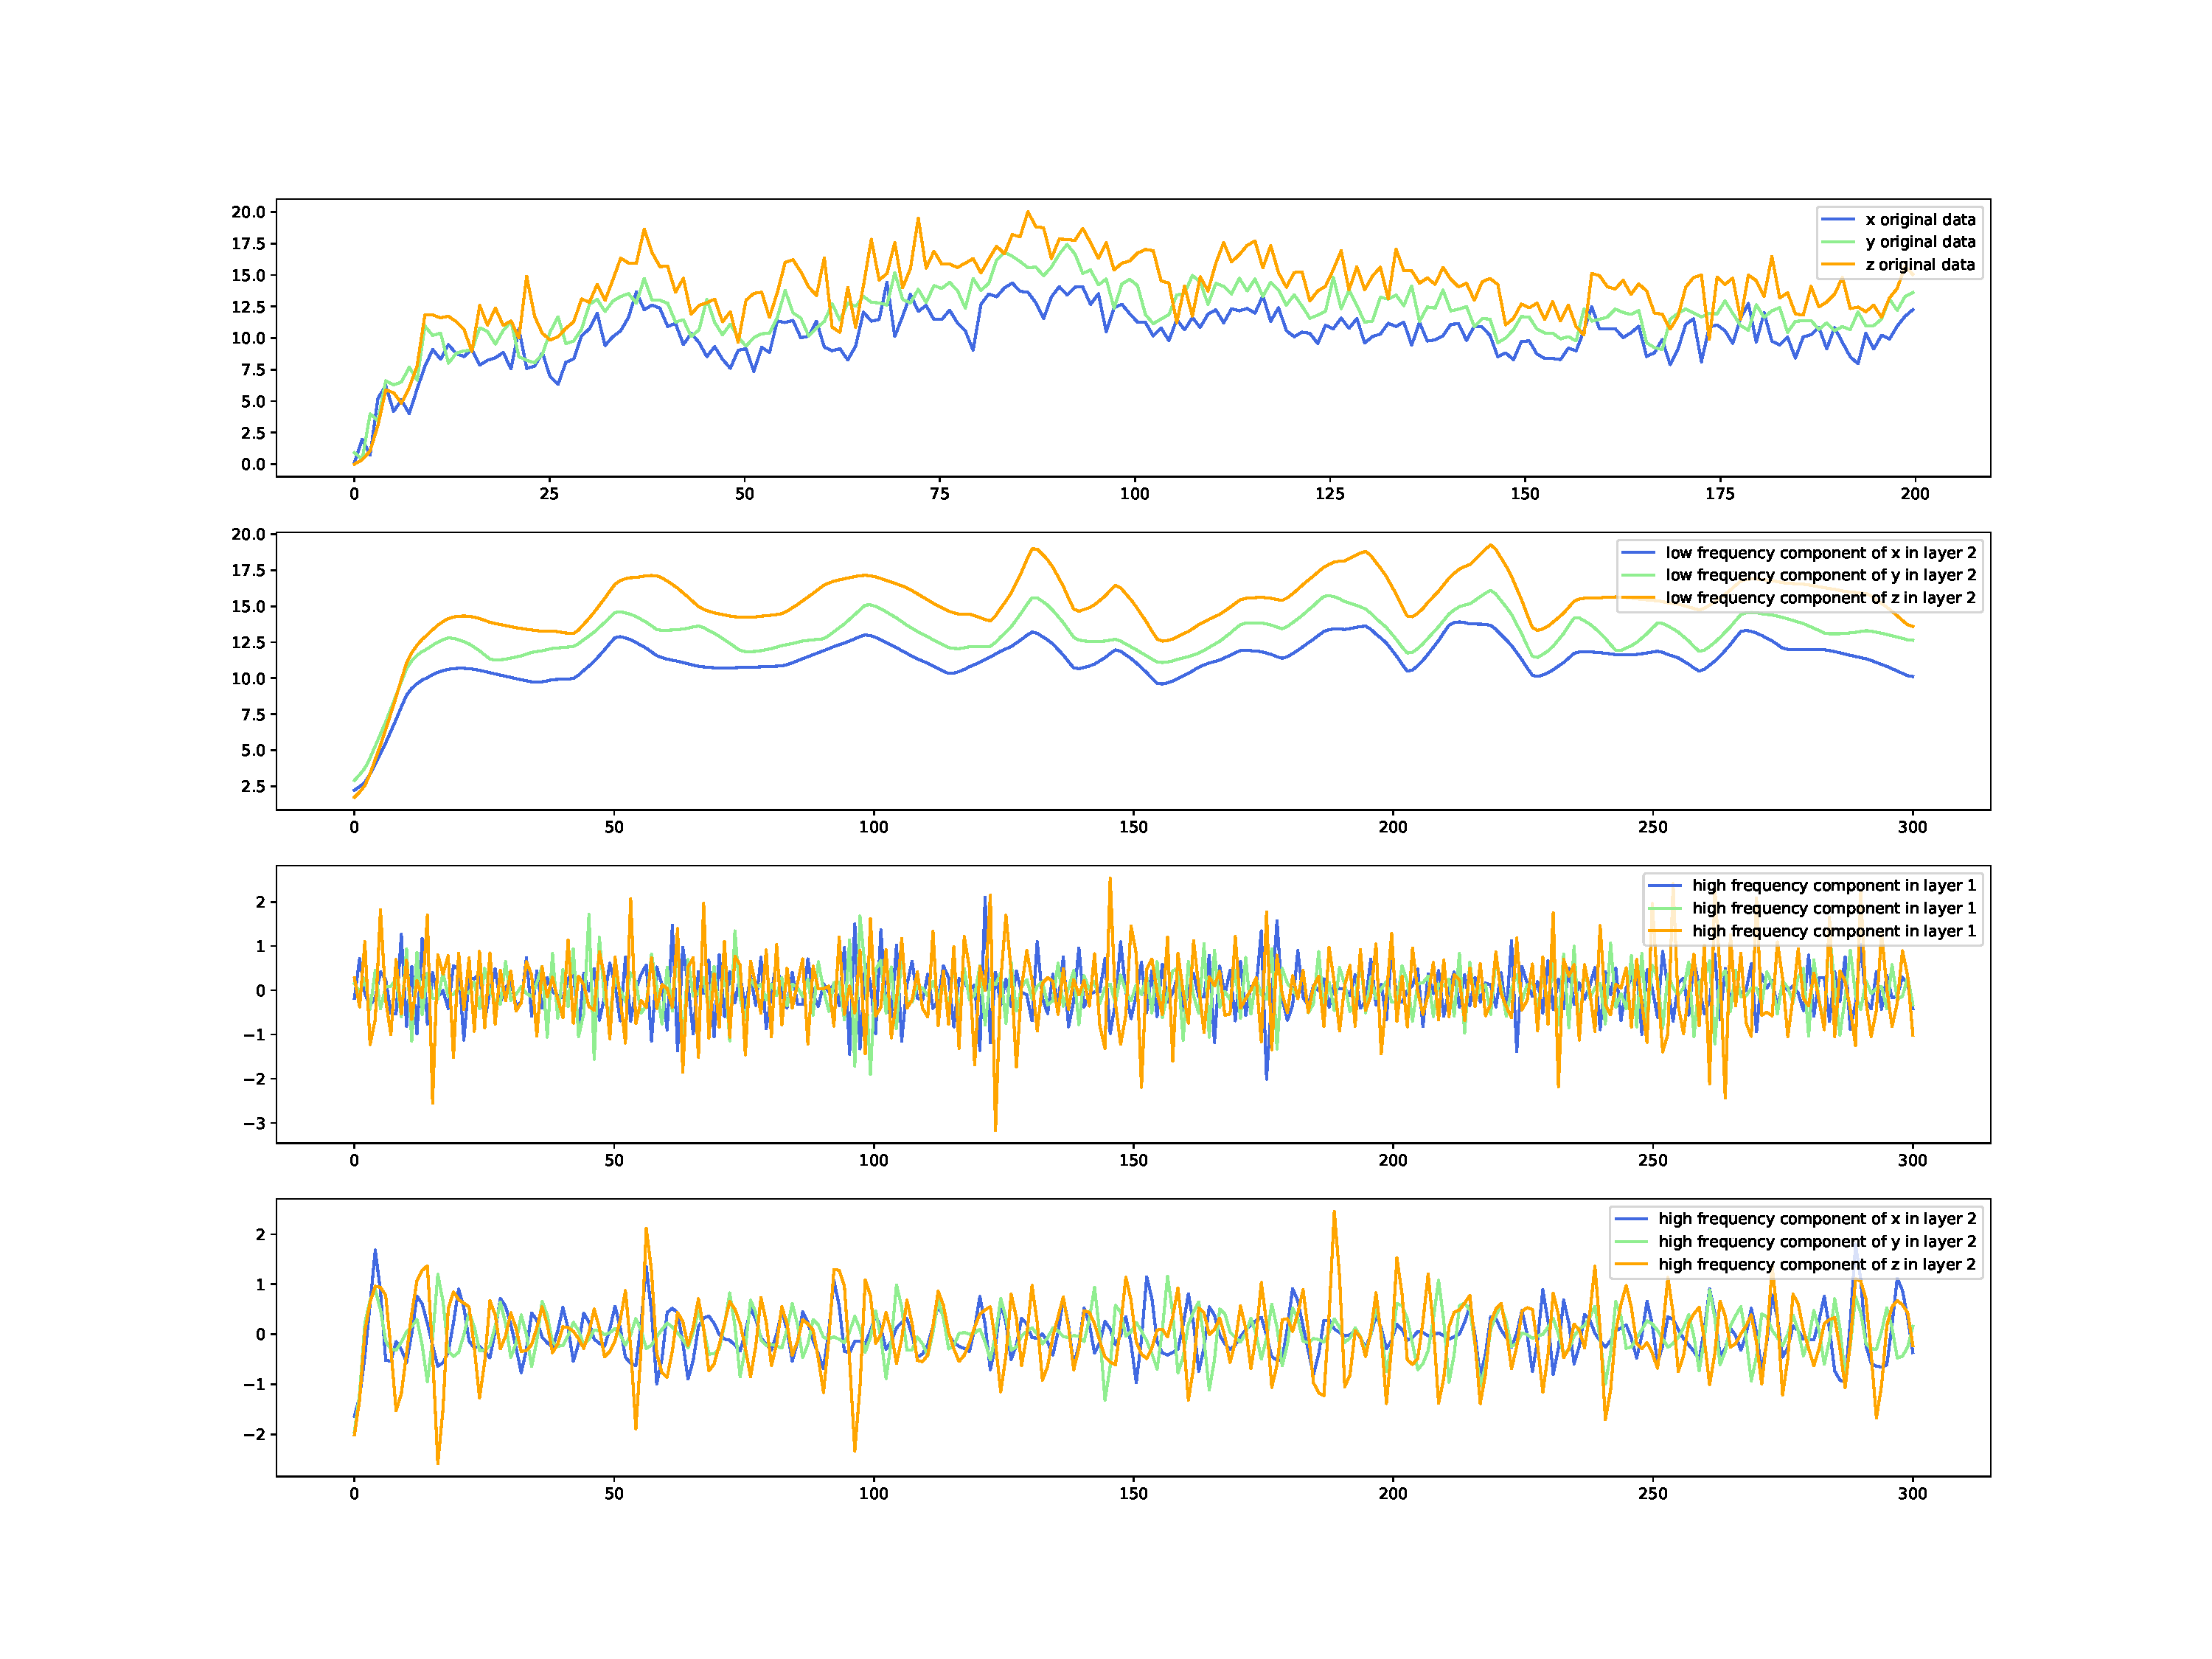
\includegraphics[width=1\textwidth]{./ch3/fig3_6.pdf}
\caption{利用ADWT模块对mVAR模型中的序列进行Symlets4小波分解。} \label{figure6}
\end{center}
\end{figure*}

对于基于MKDE的因果检测模块,RTE值与其参数$\alpha$之间及分解层数的关系如图\ref{figure7}所示,左图是已知$Z$的情况下,基于MKDE的$\rm{RTE}(X\rightarrow Y)$随参数变化的可视化,右图是已知$Z$的情况下,基于MKDE的$\rm{RTE}(Y\rightarrow X)$随参数变化的可视化,其中参数$\alpha$也设置为0.5、1、1.5和2。在\ref{figure7} (a)中,结果显示当$\alpha=0.5$时,低频段中,在已知$Z$的情况下,从$X$到$Y$的因果关系最大;而当$\alpha=1.5$时,在高频段的因果关系最大。与h\'{e}non映射的结果类似,mVAR模型中低频分量的RTE值随着$\alpha$的增大而减小。另一个不可忽略的现象是,低频分量中RTE值最统计显著时的参数是$\alpha=0.5$。这意味着在计算非平稳序列的RTE值时,应重视低概率事件,如mVAR模型中具有增长趋势的低频分量。基于h\'{e}non map和mVAR模型的RTE值与参数$\alpha$的关系的实验,本文在后面的实验中将L2层的参数设置为$\alpha=0.5$,高频分量设置为$\alpha=2$。
\begin{figure}[!ht]
\begin{center}
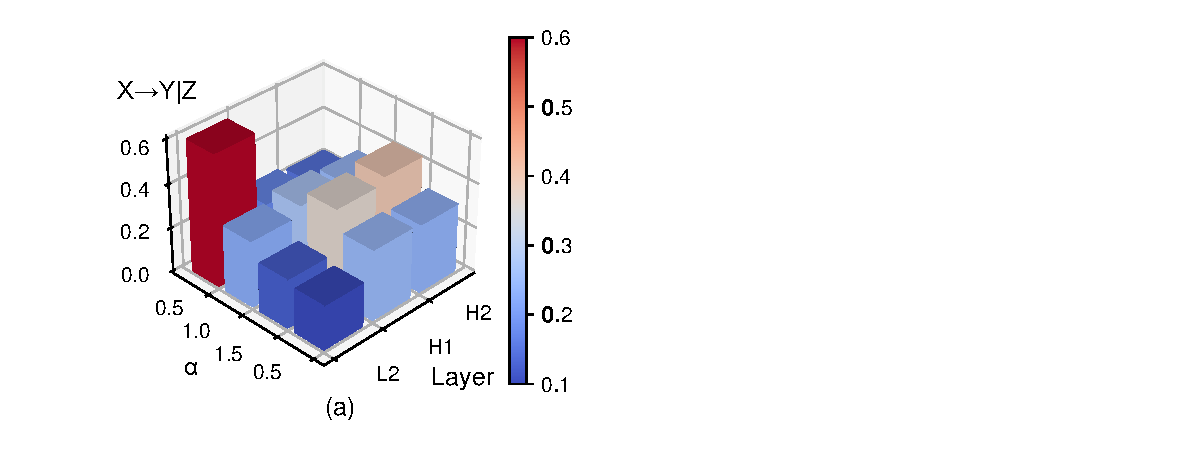
\includegraphics[scale=0.5]{./ch3/fig3_7.pdf}
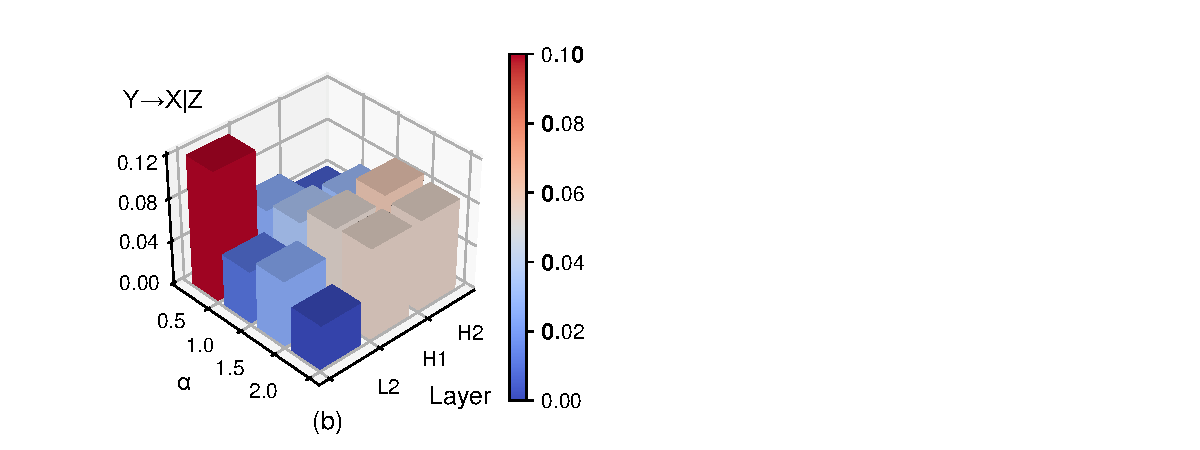
\includegraphics[scale=0.5]{./ch3/fig3_8.pdf}
\caption{基于MKDE的RTE在VAR模型上结果随参数$\alpha$的和分解层数变化的可视化。} \label{figure7}
\end{center}
\end{figure}

\subsubsection{真实数据实验}
基于合成数据的结果,我们得到了$\rm{RTE}$相关参数的先验知识,现在我们转向真实数据的实验验证。真实数据的实验也包括两部分:ADWT模块性能验证和基于 MKDE 的 RTE 效果验证。真实数据被分成两组,ADWT模块的数据分割与仿真数据实验相同。在MKDE模块的实验中,显著性检验同样采用马尔可夫块引导法(Markov block bootstrap),显著水平设置为$5\%$四分位数($p<0.05$),其中block大小也为20。方程 \eqref{TE} 中的时间延迟长度设为$l=k=5$。实验和比较结果将在本节的其余部分给出。


\textbf{实验 1: 基准数据集CauseEffectPairs}
与仿照数据实验类型,首先,我们进行了对ADWT模块的性能实验,其中分解层设置为2,不同小波函数的重构性能如表\ref{table3}所示。从表\ref{table3}中两个基准数据集的MSE结果可以看出,与原始小波相比,基于ADWT模块的所有小波函数的分解重构性能都得到了普遍提高。同时,消失矩是影响重建性能的另一个因素,高消失矩的symlets系列小波具有较好的对称性,在对两组数据进行分析和重建时可以减少相位失真。基于Symlets20的ADWT模块是所有小波函数中性能最好的。然而,在计算成本更低的情况下,Symlets4在混凝土抗压强度数据集上的重建性能并不明显劣于Symlets20,表\ref{table3}中Symlets4的方差显示了其更好的鲁棒性。因此,我们采用Symlets4对混凝土抗压强度序列进行分解,采用Symlets20对电力负荷数据进行分解。
\begin{table*}[!ht]
\centering
\fontsize{8}{14}\selectfont
\caption{ADWT模块在混凝土抗压强度(CCS)和电力负荷(EL)上的平均MSE。括号中的值为性能标准偏差。}
\begin{tabular}{lllll}
 \hline
   & \multicolumn{2}{c}{original}&  \multicolumn{2}{c}{ADWT}\\
  \hline
  Wavelet function & CCS &EL&  CCS&EL\\
  \hline
  Haar & $0.3527\ (0.1597)$ & $0.4136\ (0.0353)$& $0.1137\ (0.3919)$& $0.1754\ (0.3309)$\\
  \hline
  db4 & $0.3139\ (0.0739)$ & $0.4443\ (0.1597)$& $0.1347\ (0.1184)$& $0.1847\ (0.5512)$\\
  \hline
  db20 & $0.3035\ (0.0510)$ & $0.2759\ (0.3431)$& $0.0577\ (0.1666)$& $0.2047\ (0.3217)$\\
  \hline
  Symlets4  & $0.3570\ (0.1971)$ & $0.3841\ (0.1471)$& $0.0534\ (0.8710)$& $0.1573\ (0.0227)$\\
  \hline
  Symlets20  & $0.3135\ (0.1730)$ & $0.3158\ (0.2828)$& $0.0510\ (0.0293)$& $0.1129\ (0.0583)$\\
  \hline
\end{tabular}
\label{table3}
\end{table*}

对于因果关系检测模块的性能评估,基准数据集CauseEffectPairs提供了每个变量之间的真实因果关系,在CCS数据集中,影响因素包括:水泥含量(Cement)、高炉矿渣含量(Blast furnace slag)、粉煤灰含量(Fly ash)、水含量(Water)、超塑化剂含量(Superplasticizer)、粗集料含量(Coarse aggregate)、细集料含量(Fine aggregate)以及使用年份(Age)。所有的影响因素变量都是抗压强度的真实因果源。RTE模块生成的不同频段的因果关系如表\ref{table4}所示。按照仿真数据实验中的结果,RTE的参数$\alpha$低频分量和高频分量分别设置为0.5和1.5。$p$值小于0.05的RTE被认为具有统计意义的因果关系,并在表中加重表示。表中结果表示,在低频段中,水泥、水、使用年份对抗压强度的RTE高于显著性临界值;在高频段中,高炉矿渣、超塑化剂、粗骨料、细骨料对抗压强度的RTE高于显著性临界值。 其中,从使用年份到抗压强度的信息传递 ${\rm RTE}~(\rm{Age} \rightarrow \rm{Compressive \ strength}) = 0.3709$,从含水量到抗压强度的信息传递 ${\rm RTE}~(\rm{Water} \rightarrow \rm{Compressive \ strength}) = 0.3110$  是低频段最大的两个值,说明混凝土的龄期和水胶比是影响抗压强度变化趋势的最主要因素。 在高频段,含高炉矿渣量到抗压强度的RTE值:  ${\rm RTE}~(\rm{Blast\ furnace\ salg} \rightarrow \rm{Compressive \ strength}) = 0.2059\, 0.1919$ 在高频频段上 $(H1, H2)$ 上是最大值,这表明高炉矿渣占粘结剂总量的百分比是抗压强度波动项的最大影响因素。同时,我们还注意到龄期和水分对抗压强度在低频段和高频段都有影响。同时,除了验证MKDE模块在不同层中的性能外,我们还将其与其变体模型(不含ADWT模块)进行了比较,结果显示,变体只检测高炉矿渣和龄期对抗压强度的因果关系,这点也同样说明了ADWT模块的不可替代性。

\begin{table*}[!ht]
\centering
\caption{不同频段混凝土抗压强度与其影响因素之间的RTE值,其中括号内为$p$值,$\rightarrow$为因果关系方向。加重字段表示统计显著的因果关系。}
\fontsize{7}{14}\selectfont
\begin{tabular}{lllll}
 \hline
   & L2 &  H1& H2 &variant \\
  \hline
  Cement $\rightarrow$ Compressive strength  & $\bf{0.0714\ (0.0187)}$ & $0.2324\ (0.3610)$&$0.2024\ (0.0910)$&$0.2024\ (0.0910)$ \\
  \hline
  Blast furnace slag $\rightarrow$ Compressive strength& $\bf{0.0371\ (0.0027)}$ & $0.2059\ (0.0371)$&$0.1918\ (0.0273)$&$\bf{0.0314\ (0.0305)}$\\
  \hline
  Fly ash $\rightarrow$ Compressive strength & $\bf{0.2714\ (0.0187)}$ & $\bf{0.0024\ (0.0173)}$&$\bf{0.0013\ (0.0210)}$&$0.2715\ (0.8486)$\\
  \hline
  Water $\rightarrow$ Compressive strength & $\bf{0.3110\ (0.0372)}$ & $0.0215\ (0.0835)$&$\bf{0.0311\ (0.0254)}$&$0.3062\ (0.4136)$\\
  \hline
  Super plasticizer $\rightarrow$ Compressive strength & $\bf{0.0412\ (0.0158)}$ & $0.0514\ (0.0179)$&$0.0704\ (0.0122)$&$0.2581\ (0.3193)$\\
  \hline
  Coarse aggregate $\rightarrow$ Compressive strength& $\bf{0.0813\ (0.0369)}$ & $\bf{0.0144\ (0.0014)}$&$\bf{0.0637\ (0.0023)}$&$0.0404\ (0.7473)$\\
  \hline
  Fine aggregate $\rightarrow$ Compressive strength& $\bf{0.1073\ (0.0032)}$ & $\bf{0.2324\ (0.0010)}$&$\bf{0.3014\ (0.0110)}$&$0.0079\ (0.6751)$\\
  \hline
  Age $\rightarrow$ Compressive strength& $\bf{0.1209\ (0.0087)}$ & $\bf{0.1692\ (0.0610)}$&$\bf{0.2097\ (0.0031)}$&$\bf{0.3105\ (0.0457)}$\\
  \hline
\end{tabular}
\label{table4}
\end{table*}
同样的MKDE模块性能实验也适用于电力负荷数据集。真实的因果关系也在数据集中提供,分别是:用电时刻 $\rightarrow$ 温度, 用电时刻 $\rightarrow$ 用电量, 温度 $\rightarrow$ 用电量. 基于MKDE模块的RTE估计结果如表\ref{table5}所示。

\begin{table*}[!ht]
\centering
\caption{不同频段电力负荷与其影响因素之间的RTE值,其中括号内为$p$值,$\rightarrow$为因果关系方向。加重字段表示统计意义上的因果关系。}
\fontsize{8}{14}\selectfont
\begin{tabular}{lllll}
 \hline
   & L2 &  H1& H2 & variants \\
  \hline
  Hour $\rightarrow$  Temperature & $\bf{0.0035\ (0.0404)}$ & /\ & /\ &$0.3318\ (0.1736)$\\
  \hline
  Hour $\rightarrow$ Electricity Load& $\bf{0.3136\ (0.0349)}$ & /\ & /\ &$ 0.0055\ (0.3910)$\\
  \hline
  Temperature $\rightarrow$ Electricity Load& $ \bf{0.2075\ (0.0045)}$ & $\bf{0.2763\ (0.0060)}$ & $0.1818\ (0.0749)$ & $\bf{0.0024\ (0.0091)}$\\
  \hline
\end{tabular}
\label{table5}
\end{table*}
总的来说,基于 MKDE模块 的 RTE 估计值在真实三种因果关系上都是统计显著的,这一意味着三种因果关系都被检测到。由于小时是单调递增序列,因此在ADWT模块中不会对其进行分解。在趋势项中,用电时刻和温度是电力负荷的重要影响因素,小时的变化也会影响温度的变化。特别是, $\rm{RTE}~(\rm{Hour} \rightarrow \rm{Electricity\ Load}) = 0.3136 > \rm{RTE}~(\rm{Temperature} \rightarrow \rm{Electricity\ Load}) = 0.2075$,这表明电负荷趋势受时间变化的影响更大。这一结果背后的事实是,人类活动由一天中的时间决定,而这些活动所需的电力进一步决定了电力负荷的变化趋势。同时,温度变化也是电力负荷波动的原因,但不会影响高频段的电力负荷波动。此外,对于不带ADWT模块的变型,虽然可以检测出温度与电负荷的因果关系,但从RTE值来看,用电时刻与温度、电负荷的因果关系并不显著。

在接下来的实验中,我们还比较了基于MKDE模块和其他不同估计器计算RTE的性能,本文使用了线性估计器(\cite{3_31})和二值估计器(\cite{3_32})。首先是混凝土抗压强度数据集,以低频分量为例,混凝土抗压强度数据集的计算结果如图\ref{figure8}(a)-(c)所示,列和行的数字1-9依次表示水泥、高炉矿渣、粉煤灰、水、超塑化剂、粗骨料、细骨料和抗压强度。纵轴元素表示源变量,横轴元素表示目标变量。矩阵元素值表示从源变量到目标变量的RTE值。矩阵元素颜色越深,表示从源变量到目标变量的RTE值越高。根据原文中的观点 \cite{3_26},所有变量都会引起混凝土抗压强度的变化。所有估计值的结果都表明变量与混凝土抗压强度之间存在显著的因果关系。然而,只有基于MKDE的RTE计算的结果发现了其他变量与粉煤灰含量之间的最大因果关系,而其他两个估计器所得到的RTE忽略了这一点。我们的方法计算的结果还表明,混凝土的使用年份和含水量水是对混凝土抗压强度影响最大的两个因素。相反,基于二值估计的RTE识别出了从混凝土抗压强度到含水量、超塑化剂含量、粗骨料含量和细骨料含量的显著因果关系,这与事实有明显的冲突。此外,基于线性估计的RTE会遗漏非线性偶然性,例如,基于该估计器的RTE值检测水与其他变量的非线性因果关系,这也是违反常理的,是一个假性因果关系。


\begin{figure}[!ht]
\begin{center}
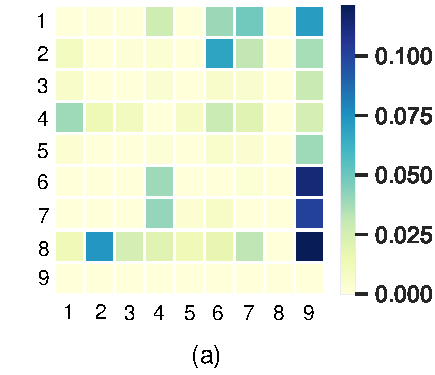
\includegraphics[scale=0.5]{./ch3/fig3_9.pdf}
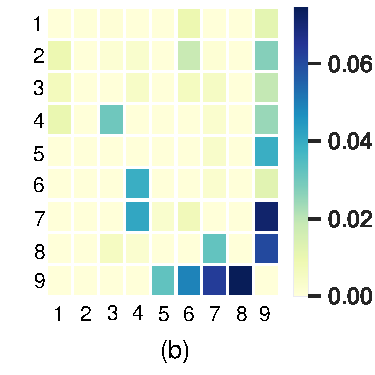
\includegraphics[scale=0.5]{./ch3/fig3_10.pdf}
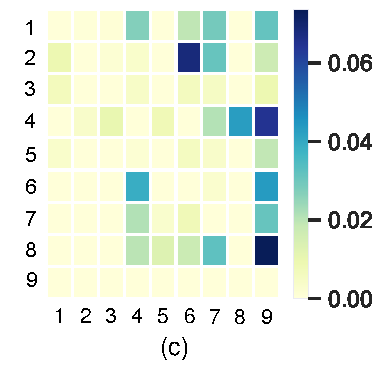
\includegraphics[scale=0.5]{./ch3/fig3_11.pdf}
\caption{不同估计器的RTE值在混凝土抗压强度数据集上的对比。(a) 基于MKDE的RTE。(b) 基于线性估计的 RTE。(c) 基于二值估计的RTE。} \label{figure8}
\end{center}
\end{figure}

接下来是电力负荷数据集上,不同估计器的RTE的比较,结果如图\ref{Figure9} (a)-(c)所示,列和行的数字1-3依次表示时刻、温度和用电负荷。纵轴元素表示源变量,水平轴元素表示目标变量。。数据集中真实的因果关系是,时刻和温度是互为因果关系的,它们都是电力负荷的原因。这可以从图\ref{Figure9} (a) MKDE模块结果可以有效地检测出共同因果关系。时刻和温度的因果关系显著高于图\ref{Figure9} (c)的结果,即bin估计器生成的RTE。同时,bin估计器给出了从电力负荷到时刻的显著RTE值,以及时刻与温度之间的显著RTE值,这些都与事实相反。这个结果说明了bin估计器在处理高耦合系统时估计假因果关系。因此,基于混凝土抗压强度和电荷载的结果,我们可以得出结论,MKDE模块可以更准确地捕捉多变量之间的因果关系。
\begin{figure}[!ht]
\begin{center}
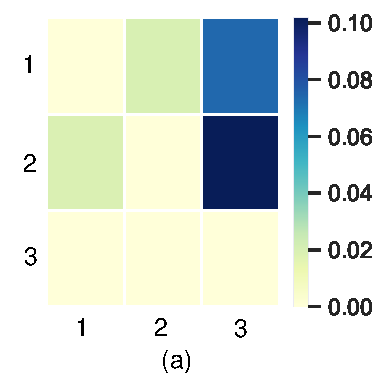
\includegraphics[scale=0.5]{./ch3/fig3_12.pdf}
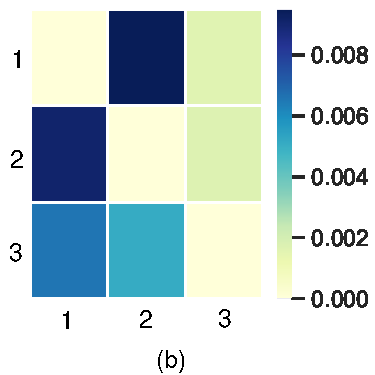
\includegraphics[scale=0.5]{./ch3/fig3_13.pdf}
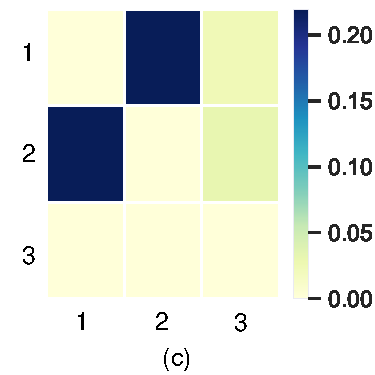
\includegraphics[scale=0.5]{./ch3/fig3_14.pdf}
\caption{不同估计器的RTE值在电力负荷数据集上的对比。(a)基于MKDE模块的RTE。(b)基于RTE的线性估计。(c)基于bin估计的RTE。} \label{Figure9}
\end{center}
\end{figure}

\textbf{实验 2: RIOHTrack 数据集}

最后,我们验证ADWT模块的性能和基于MKDE的RTE模块对来自RIOHTrack的车辙数据及其影响因素的有效性。在ADWT模块的验证中,初始设置分解层数为4,并选择Symlets20小波函数。车辙分解结果如图\ref{Figure10}所示,图中从上到下分别为:原始数据、第4层产生的低频分量、第1层、第2层、第3层和第4层产生的高频分量。

\begin{figure}[!ht]
\begin{center}
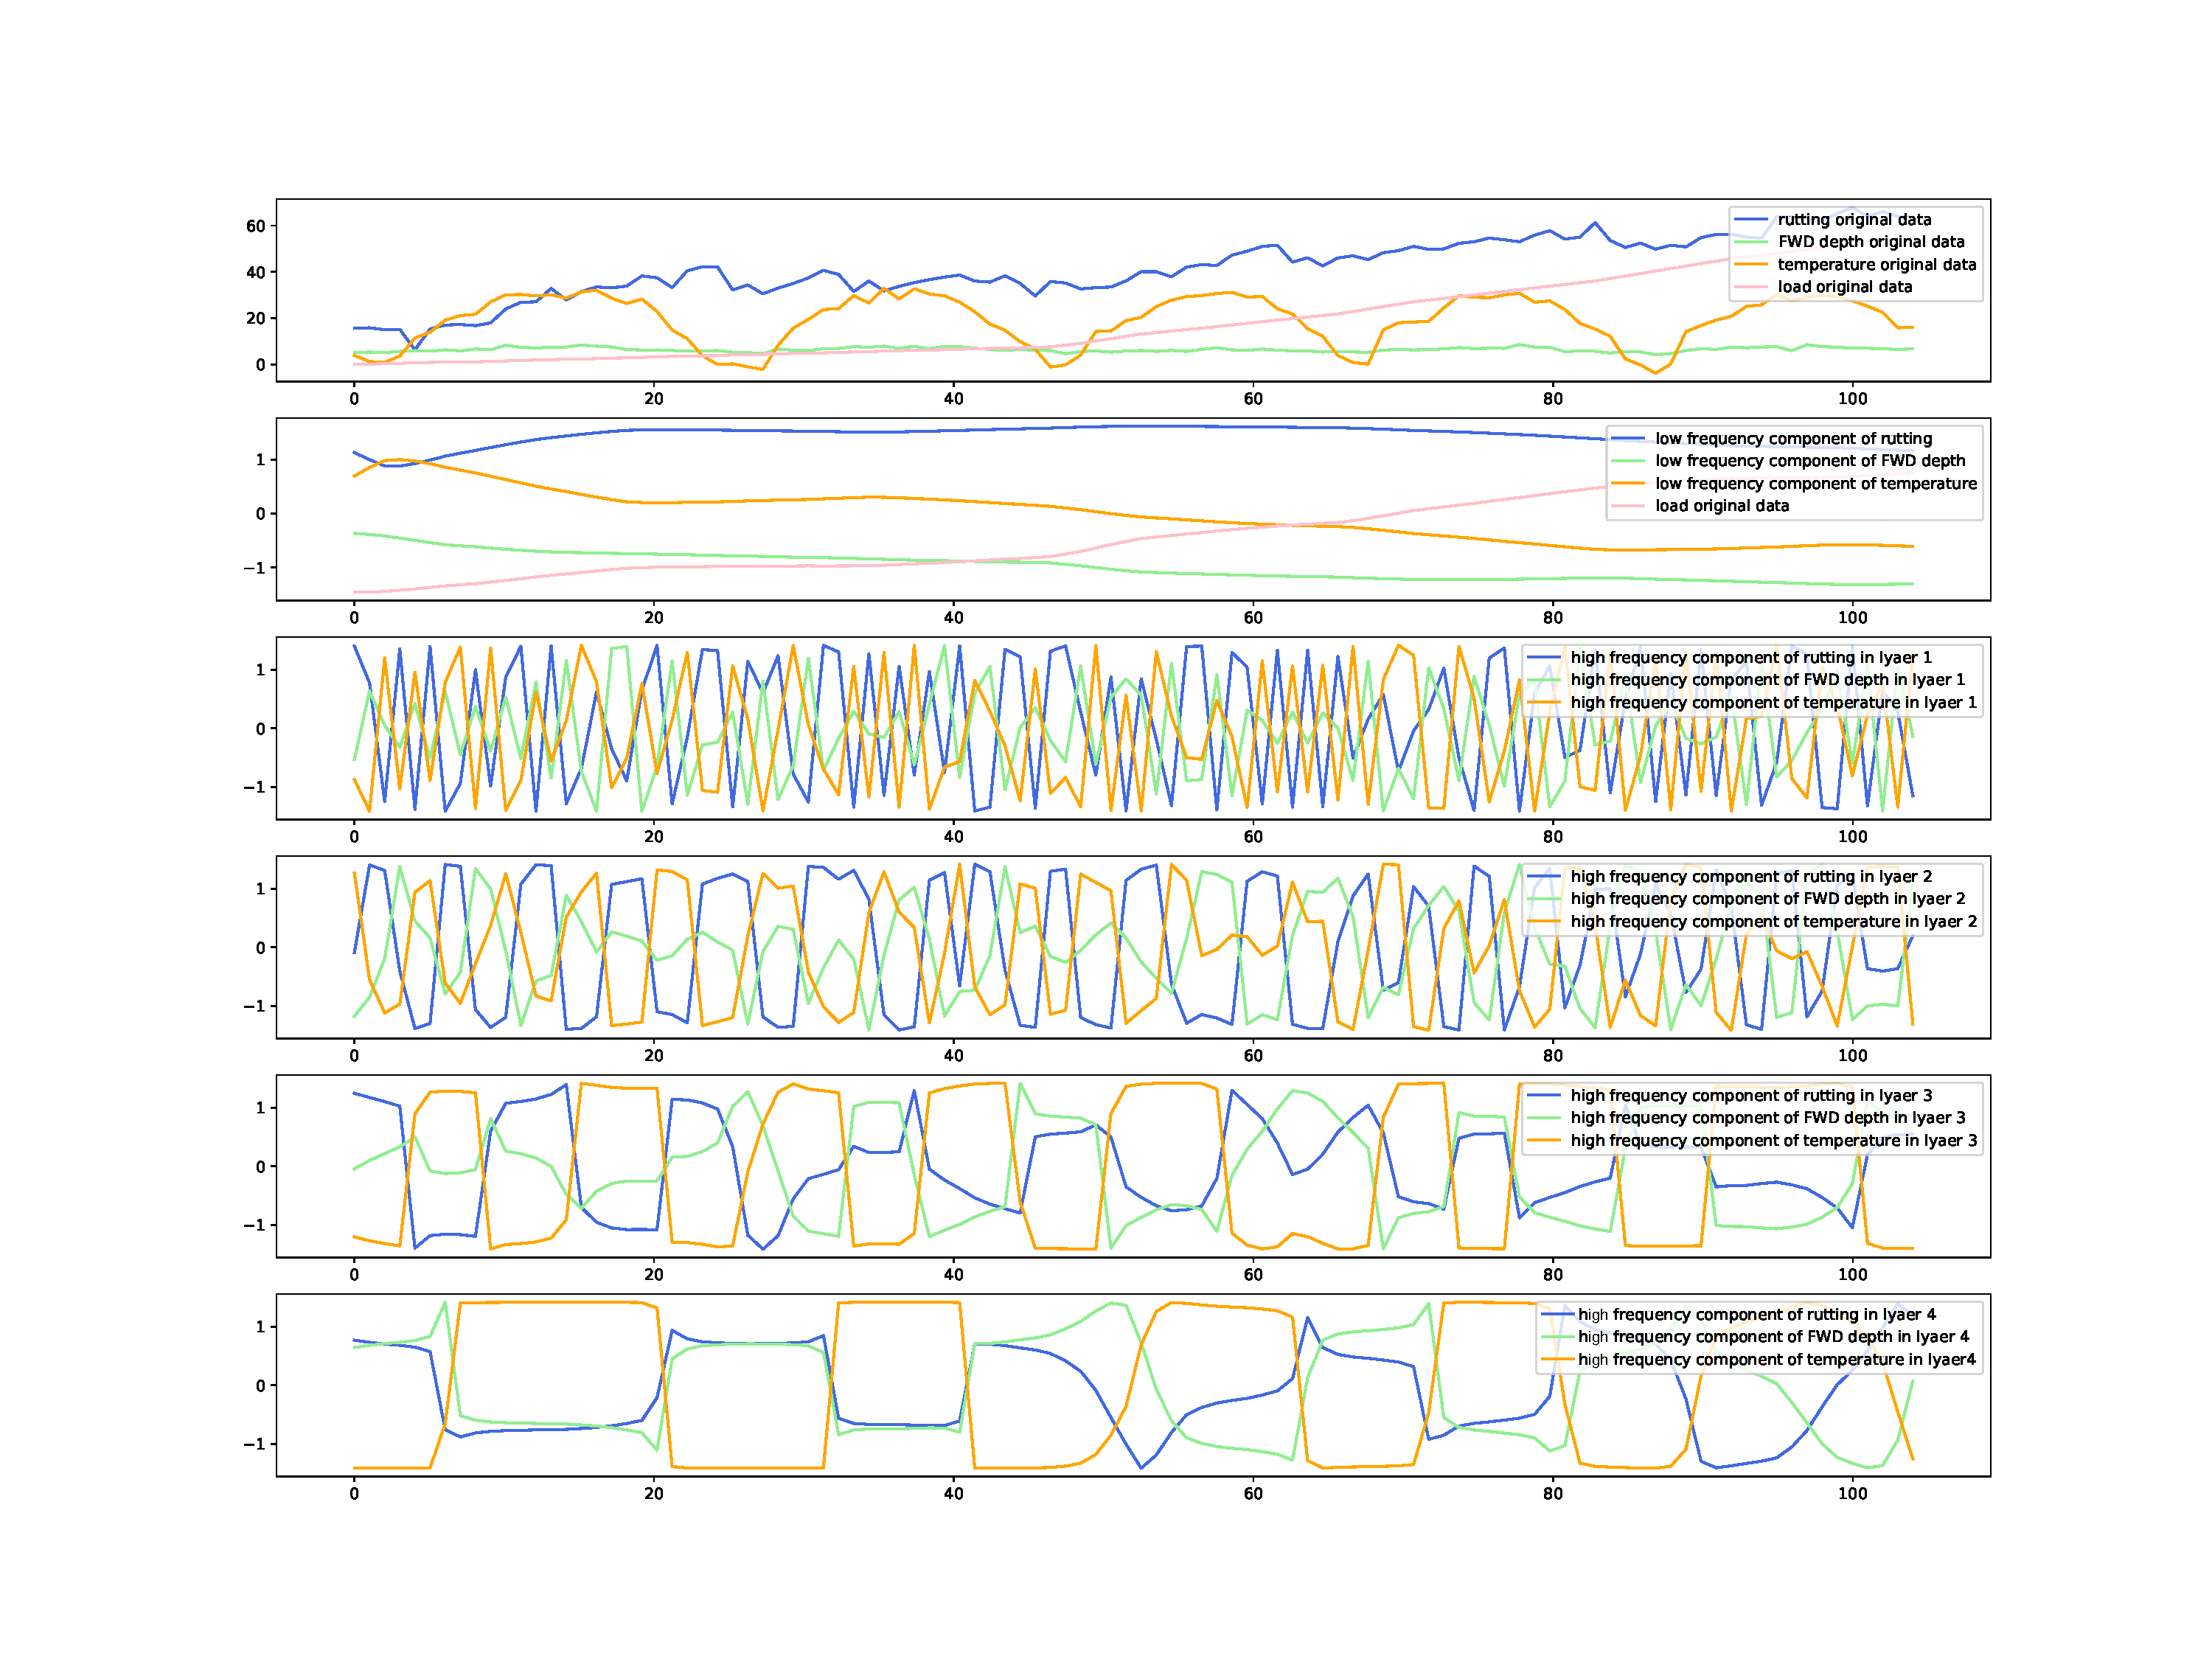
\includegraphics[scale=0.26]{./ch3/fig3_15.pdf}
\caption{利用ADWT模块对车辙及其影响因素进行Symlets20小波分解。} \label{Figure10}
\end{center}
\end{figure}

在每个分解层中,低频滤波器和高频滤波器对应的频段分别为 $(0, \frac{f_{l}}{2^{l+1}})$和$(\frac{f_{l}}{2^{l+1}},\frac{f_{l}}{2^{l}})$,其中$f_{l}$为采样频率,$l$为层数。因此,原始序列的分量被分解为5个频段:$L{4}: (0Hz-4Hz)$, $H{4}: (4Hz-8Hz)$, $H{3}: (8Hz-16Hz)$, $H{2}: (16Hz-32Hz)$, $H{1}: (32Hz-64Hz)$,其中$L{4}$代表低频段,$H{1}-H{4}$代表高频段。ADWT模块在RIOHTrack数据上的性能如表\ref{table6}所示。与仿真数据的结果一样,在ADWT模块中,消失矩阶越高的小波的mse值越高,其中Symlets20与ADWT模块的mse值最佳,为0.1039。 此外,我们还比较了上采样到原始序列长度的高频分量,度量指标为两个分量之间的mse。结果表\ref{table6_1}中所示,低频分量的变化率从第三层开始变小,到第四层高频分量几乎没有变化,这说明在更深的一层没有更多的信息被分解出来。RIOHTrack数据集中STR1路面结构在不同层的分解结果如图\ref{Figure9}所示。各变量的分解序列被归一化,映射为[0,1],以消除量纲的影响。有趣的是,车辙的高频分量、中心点挠度和温度在第4层$(4Hz-8Hz)$前40个采样周期的变化周期基本相同,在第3层$(8Hz-16Hz)$后30个采样周期的变化周期也基本相同,这预示着这些变量在这些频段可能存在因果关系。因此,在接下来的对MKDE模块的验证部分中,我们将继续关注这两个频段来验证我们的猜想。

\begin{table*}[!ht]
\centering
\caption{ADWT模块在RIOHTrack数据集上的平均重构性能,括号中的值为性能的标准偏差。}
\begin{tabular}{lll}
 \hline
  Wavelet & original &  ADWT  \\
  \hline
  Haar & $0.4943\ (0.3710)$ & $0.2751\ (0.0935)$\\
  \hline
  db4 & $0.5335\ (0.6233)$ & $0.2159\ (0.1481)$\\
  \hline
  db20 & $0.3573\ (0.3710)$ & $0.1365\ (0.1179)$\\
  \hline
  Symlets4  & $0.5228\ (0.8710)$ & $0.2021\ (0.1510)$\\
  \hline
  Symlets20  & $0.2920\ (0.1531)$ & $0.1039\ (0.0813)$\\
  \hline
\end{tabular}
\label{table6}
\end{table*}


\begin{table*}[!ht]
\centering
\caption{ADWT模块在RIOHTrack数据集上每一层平均重构性能,括号中的值为性能的标准偏差。}
\begin{tabular}{llll}
 \hline
  Wavelet  &  $L_{1}\sim L_{2}$&  $L_{2}\sim L_{3}$&  $L_{3}\sim L_{4}$ \\
  \hline
  Haar & $0.4738\ (0.2609)$ & $0.1381\ (0.1110)$& $0.0013\ (0.0105)$\\
  \hline
  db4 & $0.5141\ (0.6130)$ & $0.2173\ (0.3537)$& $0.0079\ (0.0310)$\\
  \hline
  db20 & $ 0.3299\ (0.8710)$ & $0.1818\ (0.0100)$& $0.0016\ (0.0007)$\\
  \hline
  Symlets4  & $0.4107\ (0.2310)$ & $0.1539\ (0.1710)$& $0.0031\ (0.0010)$\\
  \hline
  Symlets20  & $0.3866\ (0.1919)$ & $0.1581\ (0.2391)$& $0.0013\ (0.0126)$\\
  \hline
\end{tabular}
\label{table6_1}
\end{table*}

在RIOHTrack的MKDE模块实验部分,我们设置RTE参数$\alpha=0.5$为低频分量,$\alpha=1.5$为高频分量。根据沥青路面弹性层系理论,路面车辙与路面结构、层厚、路面力学响应等内部因素和温度、交通荷载轴线、荷载轴重等外部因素有关。影响因素对车辙产生的RTE值见表\ref{table7}和\ref{table7_1}。我们还将结果与框架变量(无ADWT)进行了比较。总的来说,本文提出的方法所确定的具有统计意义的因果关系与实际情况相吻合。特别地,三个影响因素与车辙的因果关系在低频品牌中都是显著的,这意味着它们是车辙加深趋势项的原因。并且$\rm RTE(\rm{Temperature} \rightarrow \rm{Rutting})=0.1307$为最高值,表明温度是影响轨道车辙演变趋势的最大影响因素。此外,基于MKDE的RTE值从温度和中心点挠度高频分量到车辙高频分量在第3层和第4层也是显著的,这与上一小节的推测不谋而合。有趣的是,车辙与中心点挠度在高频段具有明显的因果关系,也就是说车辙与中心点挠度在路面系统中是一对互为因果的耦合变量。相反,不含ADWT的框架仅检测到荷载与车辙之间存在显著的因果关系,没有证据表明其他变量对车辙有影响,而且中心点挠度似乎不受车辙的影响。因此,上述结果表明ADWT可以帮助框架检测RIOHTrack数据的多尺度因果关系。

\begin{table*}[!ht]
\fontsize{6}{6}\selectfont
\centering
\caption{RIOHTrack数据集在不同频段(L4-H2层)车辙与影响因素之间RTE值,括号内为$p$值,$\rightarrow$为因果关系方向。加重字段表示统计意义上的因果关系。}
\begin{tabular}{llll}
 \hline
   & L4 &  H1& H2 \\
  \hline
  Temperature $\rightarrow$  Rutting & $\bf{0.1307\ (0.0320)}$ & $\bf{0.0683\ (0.0041)}$&$0.0803\ (0.3021)$ \\
  \hline
  Load $\rightarrow$ Rutting& $\bf{0.1094\ (0.0017)}$ & /\ & /\ \\
  \hline
  CPD $\rightarrow$ Rutting& $\bf{0.1135\ (0.0217)}$ & $\bf{0.2324\ (0.0037)}$&$\bf{0.2024\ (0.0261)}$\\
  \hline
  Rutting $\rightarrow$ CPD& $\bf{0.0311\ (0.0031)}$ & $0.0164\ (0.3610)$&$\bf{0.0424\ (0.0210)}$\\
  \hline
\end{tabular}
\label{table7}
\end{table*}

\begin{table*}[!ht]
\fontsize{6}{6}\selectfont
\centering
\caption{RIOHTrack数据集在不同频段(H3-H4层)车辙与影响因素之间RTE值,括号内为$p$值,$\rightarrow$为因果关系方向。加重字段表示统计意义上的因果关系。}
\begin{tabular}{lllll}
 \hline
   & L4 & H3 & H4 & variant \\
  \hline
  Temperature $\rightarrow$  Rutting &$0.0803\ (0.3021)$ &$0.0402\ (0.0734)$&$\bf{0.0392\ (0.0210)}$&$0.0065\ (0.4910)$\\
  \hline
  Load $\rightarrow$ Rutting&  /\ & /\ & /\ &$\bf{0.1027\ (0.0010)}$\\
  \hline
  CPD $\rightarrow$ Rutting& $\bf{0.2024\ (0.0261)}$&$\bf{0.2024\ (0.0391)}$&$0.0052\ (0.0910)$&$0.0030\ (0.3907)$\\
  \hline
  Rutting $\rightarrow$ CPD& $\bf{0.0424\ (0.0210)}$&$0.1024\ (0.0535)$&$0.0076\ (0.0769)$&$0.0013\ (0.1703)$\\
  \hline
\end{tabular}
\label{table7_1}
\end{table*}
在最后的实验中,我们将基于MKDE的RTE模块的性能与上述其他两种方法,即线性估计器和bin估计进行了比较。以第4层低频分量的全部19种路面为例,基于RTE的2016-2018年和2019-2021年的因果网络分别如图\ref{Figure11}和\ref{Figure12}所示。如上所述,所有影响因素都是车辙产生的原因,车辙也是中心点挠度产生的原因。总之,图\ref{Figure11}(a)和图\ref{Figure12}(a)中的两个结果都表明MKDE模块能够有效地检测出各变量之间的显著因果关系。对于基于线性估计的RTE,如图\ref{Figure11}(b)所示,车辙深度与中心点挠度之间的因果关系未被检测到,两个周期内温度与中心点挠度之间的因果关系均被忽略。图\ref{Figure11}(c)和图\ref{Figure12}(c)中的结果表明,bin估计器识别出了荷载与温度之间的强因果关系,这显然是一个错误的结论。此外,两组结果为RIOHTrack的因果检测提供了重要启示,后期中心点挠度与车辙波动项的因果关系显著低于前期,而线性发展的交通荷载与车辙的因果关系变得更强。这些结论与车辙演变三阶段理论相一致,结果证明了本章提出的ADWTRTE的有效性,也为进一步表征车辙演变动力学模型提供了理论依据。至此,对于本章提出的ADWTRTE所有的实验完成,结果验证了本章所提出的方法的有效性与健壮性。

\begin{figure}[H]
\begin{center}
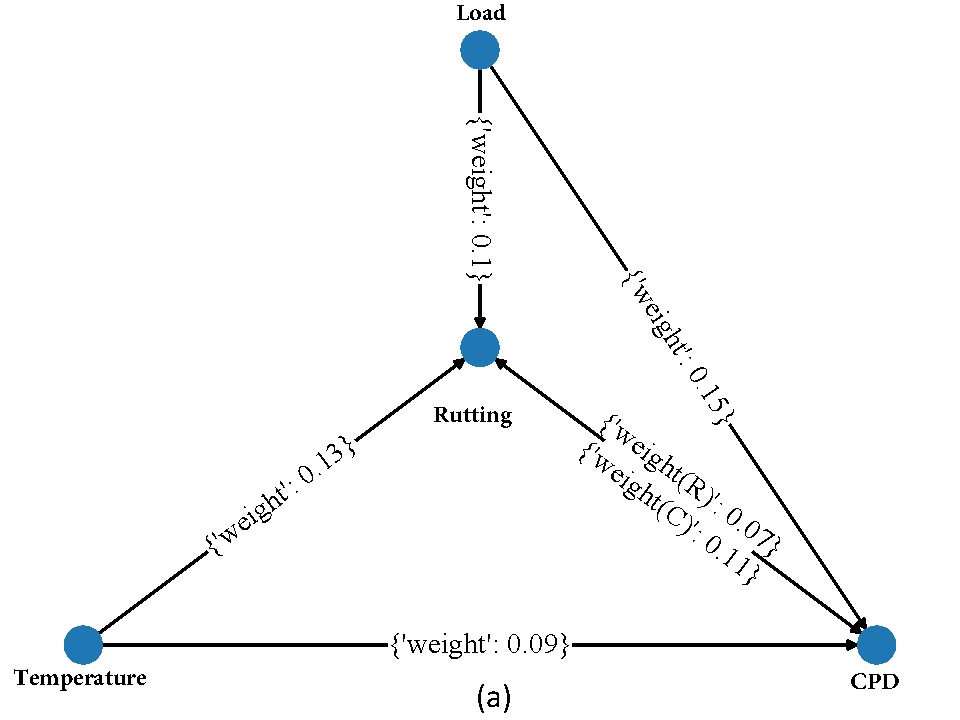
\includegraphics[scale=0.3]{./ch3/fig3_16.pdf}
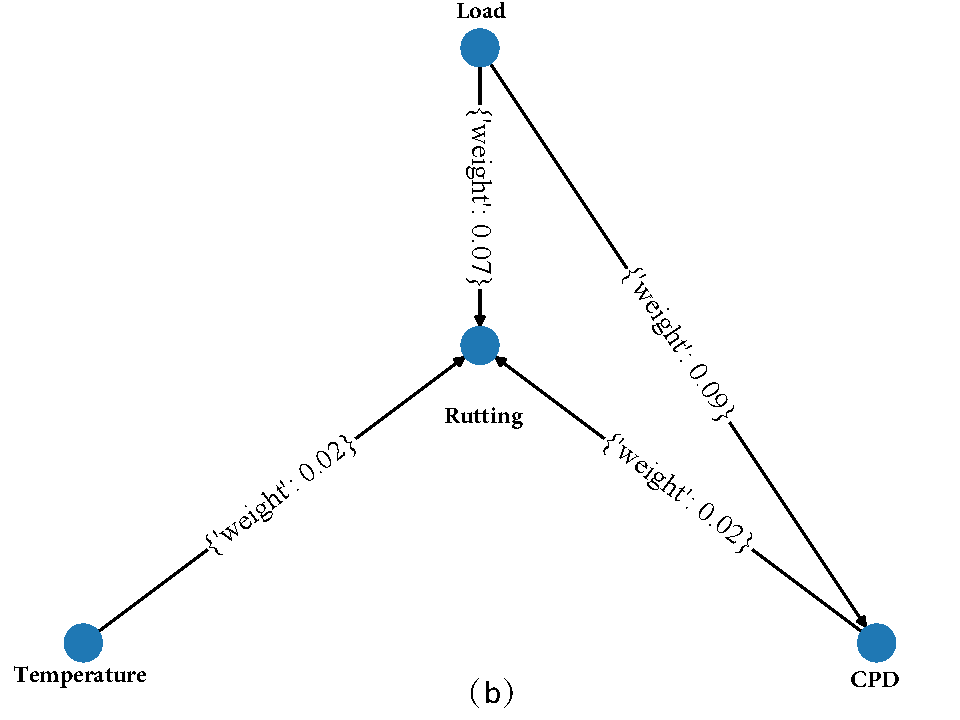
\includegraphics[scale=0.3]{./ch3/fig3_17.pdf}
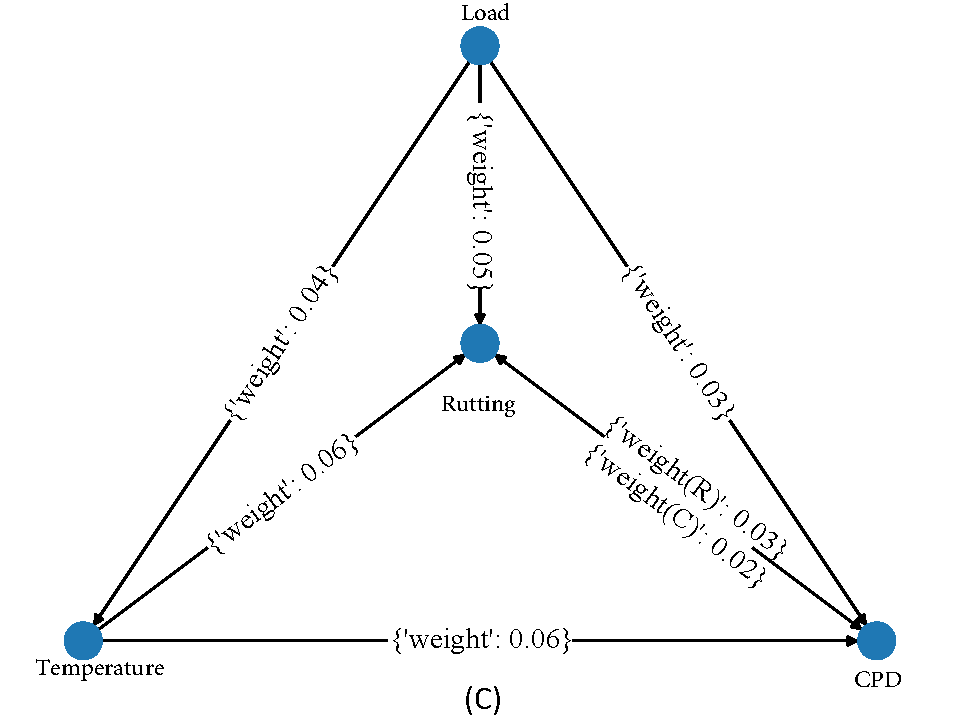
\includegraphics[scale=0.3]{./ch3/fig3_18.pdf}
\caption{2016-2018年RIOHTrack数据集上车辙及其影响因素间,不同估计器生成的RTE值比较。(a) 基于MKDE模块的RTE。(b) 基于线性估计的RTE。(c) 基于二进制估计的RTE。} \label{Figure11}
\end{center}
\end{figure}
\begin{figure}[H]
\begin{center}
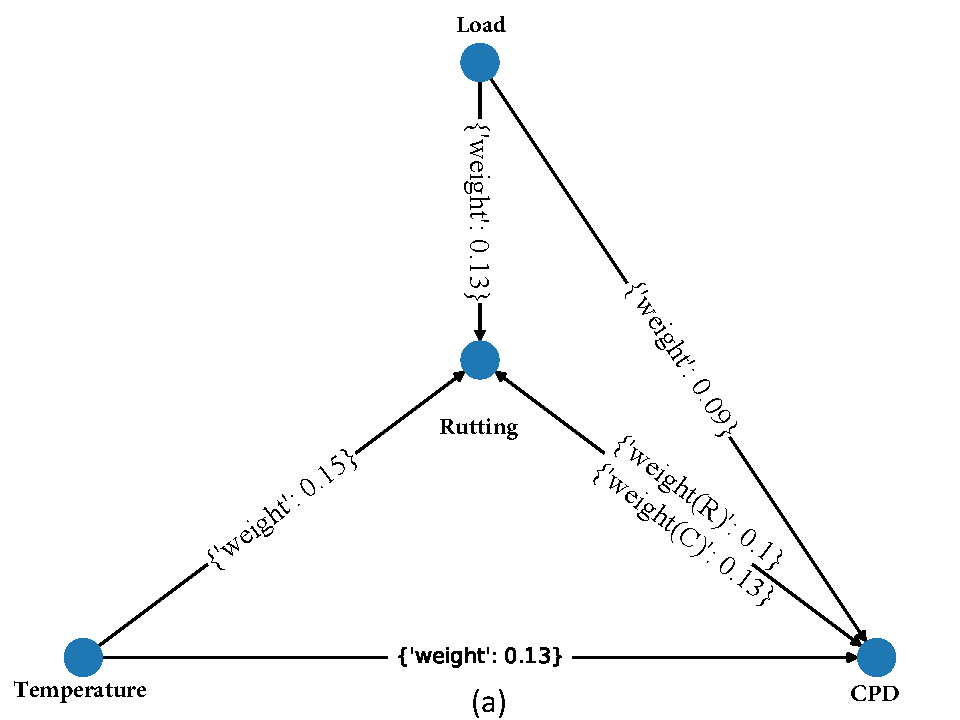
\includegraphics[scale=0.3]{./ch3/fig3_19.pdf}
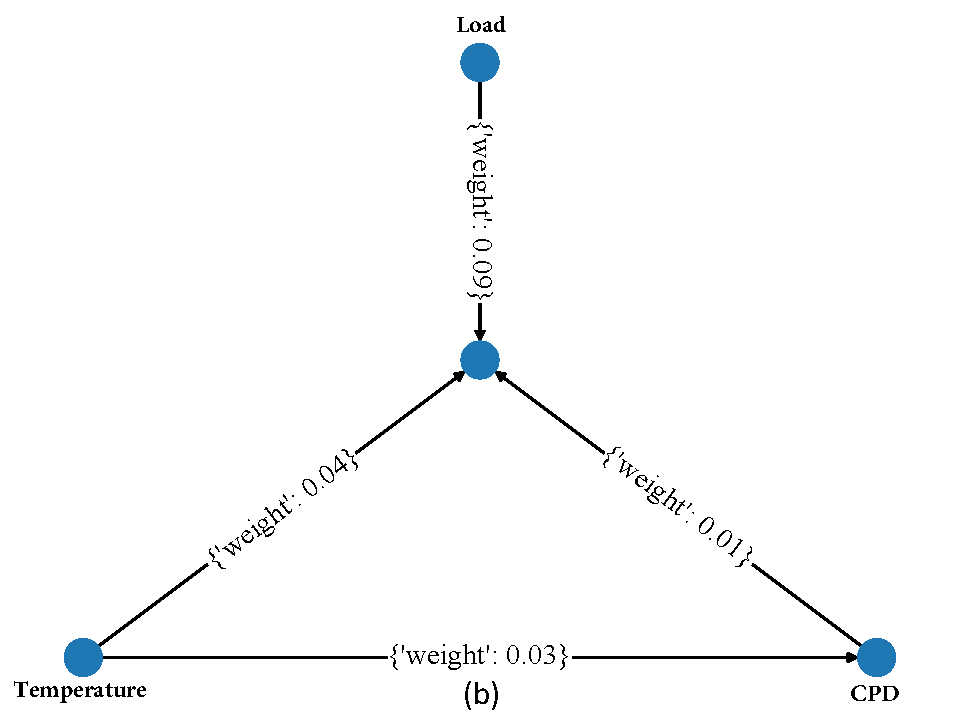
\includegraphics[scale=0.3]{./ch3/fig3_20.pdf}
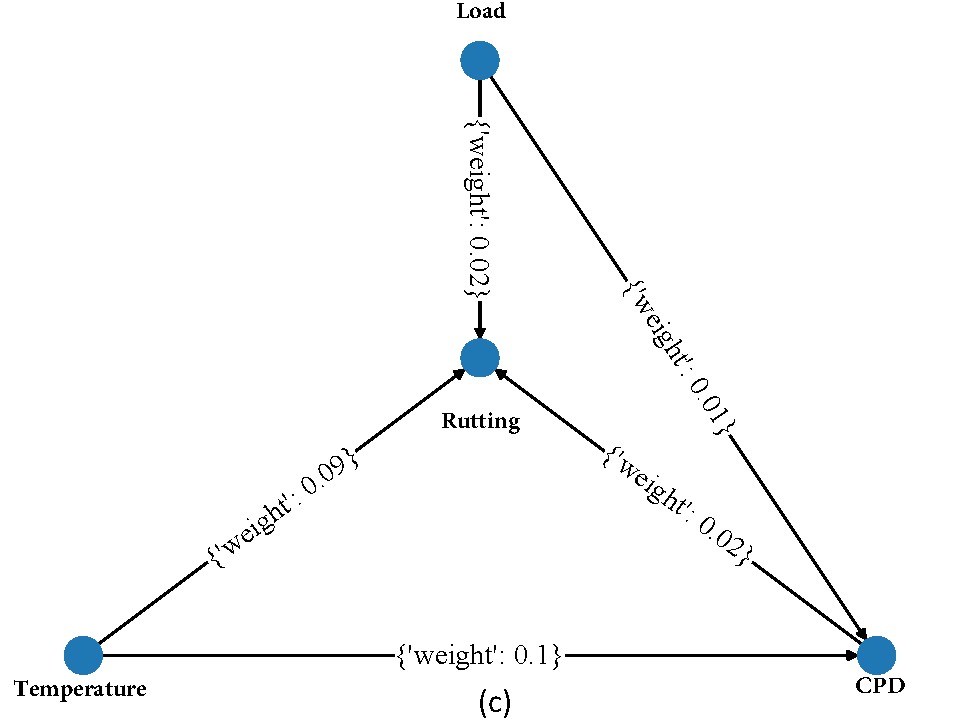
\includegraphics[scale=0.3]{./ch3/fig3_21.pdf}
\caption{2018-2021年RIOHTrack数据集上车辙及其影响因素间,不同估计器生成的RTE值比较。(a) 基于MKDE模块的RTE。(b) 基于线性估计的RTE。(c) 基于二进制估计的RTE。} \label{Figure12}
\end{center}
\end{figure}


\section{小结} 
在基于r\'{e}nyi传递熵的因果检测模型研究中,如何更准确地估计r\'{e}nyi传递熵以及如何度量多层系统的因果关系是许多学者关注的问题。针对这两个问题,本文提出了一种基于核密度估计的新型多尺度RTE方法。该方法包括两个部分: 基于ADWT的时间序列分解和基于MKDE的因果网络生成。该方法的流程是将复杂系统的所有变量作为输入,通过ADWT模块计算出最优小波系数。这些系数用于将原始时间序列分解为多层高频和低频分量,分别对应波动项和趋势项。本文用变量邻接矩阵表示系统内变量的因果关系。变量邻接矩阵由最后一层的低频分量和每一层的高频分量组成。矩阵中的节点表示系统的变量,边表示变量之间的因果关系,由MKDE模块确定。每一层的因果网络就是该方法的输出结果。具体来说,在基于ADWT的时间序列分解中,设计了一个最优小波系数的自动编码器框架,以减少分解过程中的信息损伤。自动编码器框架由小波函数组成,通过最小化原始时间和重构时间序列之间的均方误差,在编码器-解码器中训练最优小波系数。在基于MKDE的因果网络生成中,RTE值由KDE估计,KDE的核函数由最优带宽选择决定,KDE通过最小化概率密度分布与核函数之间的AMISE来测量。为了验证本研究中提出的方法的有效性,设计了一系列实验,在合成数据和真实数据上测试该模型。进行这些实验的目的是评估模型在各种情况和不同条件下的性能。合成数据使用多种参数生成,而真实数据则从多个不同来源收集。在使用合成数据进行验证时,我们进行了实验来研究ADWT模块在不同小波上重建序列的性能。我们的研究结果表明,ADWT模块能够有效降低重建数据与原始数据之间的误差。随后,我们探讨了参数$\alpha$的选择对基于RTE的因果关系检测的影响。在真实数据的验证中,我们对ADWT的性能进行了评估,并确定了在该数据上性能最好的小波基。最后,我们利用本文提出的方法构建了基于RTE值的因果网络,并利用不同的估计方法比较了因果网络构建的效果。研究结果表明,该方法在处理合成数据和真实数据时都非常有效,非常适合因果检测领域的一系列应用。
本章结果已发表在国际刊物  Neural Networks 上。具体详见作者发表论文的清单。
